\documentclass[twoside]{book}

% Packages required by doxygen
\usepackage{fixltx2e}
\usepackage{calc}
\usepackage{doxygen}
\usepackage[export]{adjustbox} % also loads graphicx
\usepackage{graphicx}
\usepackage[utf8]{inputenc}
\usepackage{makeidx}
\usepackage{multicol}
\usepackage{multirow}
\PassOptionsToPackage{warn}{textcomp}
\usepackage{textcomp}
\usepackage[nointegrals]{wasysym}
\usepackage[table]{xcolor}

% Font selection
\usepackage[T1]{fontenc}
\usepackage[scaled=.90]{helvet}
\usepackage{courier}
\usepackage{amssymb}
\usepackage{sectsty}
\renewcommand{\familydefault}{\sfdefault}
\allsectionsfont{%
  \fontseries{bc}\selectfont%
  \color{darkgray}%
}
\renewcommand{\DoxyLabelFont}{%
  \fontseries{bc}\selectfont%
  \color{darkgray}%
}
\newcommand{\+}{\discretionary{\mbox{\scriptsize$\hookleftarrow$}}{}{}}

% Page & text layout
\usepackage{geometry}
\geometry{%
  a4paper,%
  top=2.5cm,%
  bottom=2.5cm,%
  left=2.5cm,%
  right=2.5cm%
}
\tolerance=750
\hfuzz=15pt
\hbadness=750
\setlength{\emergencystretch}{15pt}
\setlength{\parindent}{0cm}
\setlength{\parskip}{3ex plus 2ex minus 2ex}
\makeatletter
\renewcommand{\paragraph}{%
  \@startsection{paragraph}{4}{0ex}{-1.0ex}{1.0ex}{%
    \normalfont\normalsize\bfseries\SS@parafont%
  }%
}
\renewcommand{\subparagraph}{%
  \@startsection{subparagraph}{5}{0ex}{-1.0ex}{1.0ex}{%
    \normalfont\normalsize\bfseries\SS@subparafont%
  }%
}
\makeatother

% Headers & footers
\usepackage{fancyhdr}
\pagestyle{fancyplain}
\fancyhead[LE]{\fancyplain{}{\bfseries\thepage}}
\fancyhead[CE]{\fancyplain{}{}}
\fancyhead[RE]{\fancyplain{}{\bfseries\leftmark}}
\fancyhead[LO]{\fancyplain{}{\bfseries\rightmark}}
\fancyhead[CO]{\fancyplain{}{}}
\fancyhead[RO]{\fancyplain{}{\bfseries\thepage}}
\fancyfoot[LE]{\fancyplain{}{}}
\fancyfoot[CE]{\fancyplain{}{}}
\fancyfoot[RE]{\fancyplain{}{\bfseries\scriptsize Generated by Doxygen }}
\fancyfoot[LO]{\fancyplain{}{\bfseries\scriptsize Generated by Doxygen }}
\fancyfoot[CO]{\fancyplain{}{}}
\fancyfoot[RO]{\fancyplain{}{}}
\renewcommand{\footrulewidth}{0.4pt}
\renewcommand{\chaptermark}[1]{%
  \markboth{#1}{}%
}
\renewcommand{\sectionmark}[1]{%
  \markright{\thesection\ #1}%
}

% Indices & bibliography
\usepackage{natbib}
\usepackage[titles]{tocloft}
\setcounter{tocdepth}{3}
\setcounter{secnumdepth}{5}
\makeindex

% Hyperlinks (required, but should be loaded last)
\usepackage{ifpdf}
\ifpdf
  \usepackage[pdftex,pagebackref=true]{hyperref}
\else
  \usepackage[ps2pdf,pagebackref=true]{hyperref}
\fi
\hypersetup{%
  colorlinks=true,%
  linkcolor=blue,%
  citecolor=blue,%
  unicode%
}

% Custom commands
\newcommand{\clearemptydoublepage}{%
  \newpage{\pagestyle{empty}\cleardoublepage}%
}

\usepackage{caption}
\captionsetup{labelsep=space,justification=centering,font={bf},singlelinecheck=off,skip=4pt,position=top}

%===== C O N T E N T S =====

\begin{document}

% Titlepage & ToC
\hypersetup{pageanchor=false,
             bookmarksnumbered=true,
             pdfencoding=unicode
            }
\pagenumbering{alph}
\begin{titlepage}
\vspace*{7cm}
\begin{center}%
{\Large Bulb \\[1ex]\large 1.\+1 }\\
\vspace*{1cm}
{\large Generated by Doxygen 1.8.14}\\
\end{center}
\end{titlepage}
\clearemptydoublepage
\pagenumbering{roman}
\tableofcontents
\clearemptydoublepage
\pagenumbering{arabic}
\hypersetup{pageanchor=true}

%--- Begin generated contents ---
\chapter{Hierarchical Index}
\section{Class Hierarchy}
This inheritance list is sorted roughly, but not completely, alphabetically\+:\begin{DoxyCompactList}
\item object\begin{DoxyCompactList}
\item \contentsline{section}{sql\+\_\+client.\+Sql\+Client}{\pageref{classsql__client_1_1_sql_client}}{}
\item \contentsline{section}{streamer.\+Streamer}{\pageref{classstreamer_1_1_streamer}}{}
\item \contentsline{section}{train.\+Trainer}{\pageref{classtrain_1_1_trainer}}{}
\item \contentsline{section}{user.\+User}{\pageref{classuser_1_1_user}}{}
\end{DoxyCompactList}
\end{DoxyCompactList}

\chapter{Class Index}
\section{Class List}
Here are the classes, structs, unions and interfaces with brief descriptions\+:\begin{DoxyCompactList}
\item\contentsline{section}{\mbox{\hyperlink{classsql__client_1_1_sql_client}{sql\+\_\+client.\+Sql\+Client}} }{\pageref{classsql__client_1_1_sql_client}}{}
\item\contentsline{section}{\mbox{\hyperlink{classstreamer_1_1_streamer}{streamer.\+Streamer}} }{\pageref{classstreamer_1_1_streamer}}{}
\item\contentsline{section}{\mbox{\hyperlink{classtrain_1_1_trainer}{train.\+Trainer}} }{\pageref{classtrain_1_1_trainer}}{}
\item\contentsline{section}{\mbox{\hyperlink{classuser_1_1_user}{user.\+User}} }{\pageref{classuser_1_1_user}}{}
\end{DoxyCompactList}

\chapter{Class Documentation}
\hypertarget{classsql__client_1_1_sql_client}{}\section{sql\+\_\+client.\+Sql\+Client Class Reference}
\label{classsql__client_1_1_sql_client}\index{sql\+\_\+client.\+Sql\+Client@{sql\+\_\+client.\+Sql\+Client}}
Inheritance diagram for sql\+\_\+client.\+Sql\+Client\+:\begin{figure}[H]
\begin{center}
\leavevmode
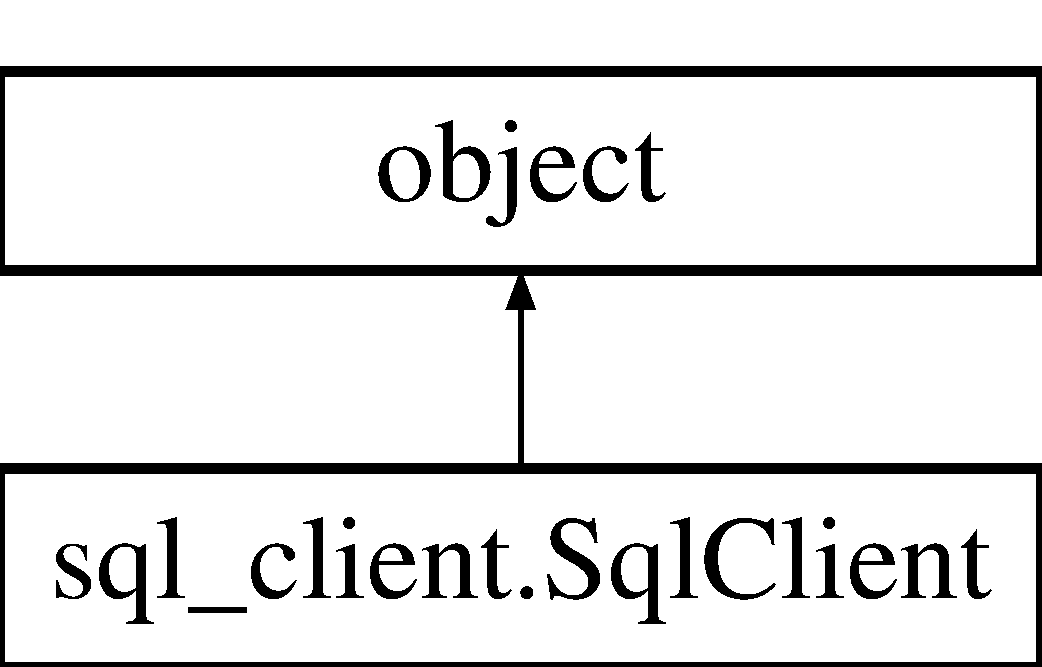
\includegraphics[height=2.000000cm]{classsql__client_1_1_sql_client}
\end{center}
\end{figure}
\subsection*{Public Member Functions}
\begin{DoxyCompactItemize}
\item 
def \mbox{\hyperlink{classsql__client_1_1_sql_client_a6800fef274fbc6b3f5f27fe2e69aa4f0}{\+\_\+\+\_\+init\+\_\+\+\_\+}} (self)
\item 
def \mbox{\hyperlink{classsql__client_1_1_sql_client_aa2dae62cb52cef01e2023a00e3abeeab}{open\+Cursor}} (self)
\item 
def \mbox{\hyperlink{classsql__client_1_1_sql_client_a19f3afe71ef8d46c5c364b9e5727b681}{close\+Cursor}} (self)
\item 
def \mbox{\hyperlink{classsql__client_1_1_sql_client_a5c2da9bb6e47f3f316e3fff6c34bc70e}{set\+Hashtag}} (self, hashtag)
\item 
def \mbox{\hyperlink{classsql__client_1_1_sql_client_ab8870e714acfd8d94d5f2d632447725f}{insert\+Post}} (self, post, top\+Post=False)
\item 
def \mbox{\hyperlink{classsql__client_1_1_sql_client_a18816b3e7e51cc678cec67b3b85ebb5d}{insert\+User\+Feed}} (self, feed)
\item 
def \mbox{\hyperlink{classsql__client_1_1_sql_client_a6c838651c15d3d7484c7082dc1377be0}{insert\+User}} (self, user)
\item 
def \mbox{\hyperlink{classsql__client_1_1_sql_client_a2266364e6779025ae03f25ef42a056be}{insert\+Comments}} (self, post\+\_\+id, comments)
\item 
def \mbox{\hyperlink{classsql__client_1_1_sql_client_aeb4b2806e4055304d7005ac2173b7453}{insert\+Likers}} (self, post\+\_\+id, likers)
\item 
def \mbox{\hyperlink{classsql__client_1_1_sql_client_a5bacb4e196cb6addb7b1c2c7e1c92c4f}{set\+Label}} (self, username, label)
\item 
def \mbox{\hyperlink{classsql__client_1_1_sql_client_a1f19e8375847e847b0c0dc13dd4930c3}{get\+Username\+Urls}} (self, labeled=True, randomized=True, sponsored\+\_\+only=True)
\item 
def \mbox{\hyperlink{classsql__client_1_1_sql_client_aabd735d4f088517fb4354be42713a65d}{get\+User}} (self, username)
\item 
def \mbox{\hyperlink{classsql__client_1_1_sql_client_ae5bd5fba97db2686788dbd05cca758c4}{get\+User\+Posts}} (self, \+\_\+id)
\item 
def \mbox{\hyperlink{classsql__client_1_1_sql_client_a40842f3f655d0256a1accdec40e731b4}{get\+Users}} (self, limit, labeled=True)
\item 
def \mbox{\hyperlink{classsql__client_1_1_sql_client_a4ec5854106ec0e7cfeccfdd3e51a1653}{get\+User\+Names}} (self, limit, labeled=True)
\item 
def \mbox{\hyperlink{classsql__client_1_1_sql_client_a3d816cc763f7bfc338661b48f045ef45}{get\+Comments}} (self, post\+\_\+id)
\item 
def \mbox{\hyperlink{classsql__client_1_1_sql_client_af4d17e7a095ea153202ad62ab4400a1a}{get\+All\+Likes}} (self, n=0)
\item 
def \mbox{\hyperlink{classsql__client_1_1_sql_client_aa74c78382113ffc2204b6361e9c1d1f4}{get\+User\+Post\+Comments}} (self, user\+\_\+id)
\item 
def \mbox{\hyperlink{classsql__client_1_1_sql_client_a6f0328bf169e37403176157b9899603e}{get\+Average\+Followers\+Per\+User}} (self)
\item 
def \mbox{\hyperlink{classsql__client_1_1_sql_client_a7db4bd36f417ef6e04c27bb3c225ced7}{get\+Average\+Followings\+Per\+User}} (self)
\item 
def \mbox{\hyperlink{classsql__client_1_1_sql_client_aba9982883d49d334c0f6f2d9c7ce4965}{get\+Average\+Likes\+Per\+Post}} (self)
\item 
def \mbox{\hyperlink{classsql__client_1_1_sql_client_a21df01dcb35afd430c1e03623d393227}{get\+Average\+Comments\+Per\+Post}} (self)
\item 
def \mbox{\hyperlink{classsql__client_1_1_sql_client_a17678dbe8928fffbcb625bbdf33786c6}{get\+Hashtags\+Details}} (self)
\item 
def \mbox{\hyperlink{classsql__client_1_1_sql_client_ada4e31012fee403ce53f35564505fcc1}{get\+All\+Comments}} (self)
\item 
def \mbox{\hyperlink{classsql__client_1_1_sql_client_ab74d313a5b3e9a155fd0ad64bd22a1df}{close}} (self)
\end{DoxyCompactItemize}
\subsection*{Public Attributes}
\begin{DoxyCompactItemize}
\item 
\mbox{\Hypertarget{classsql__client_1_1_sql_client_a23b9856c2aa3bbb39027108647fa9736}\label{classsql__client_1_1_sql_client_a23b9856c2aa3bbb39027108647fa9736}} 
{\bfseries config}
\item 
\mbox{\Hypertarget{classsql__client_1_1_sql_client_af82ec6f9b2b4383b2e7ef66731bdf03f}\label{classsql__client_1_1_sql_client_af82ec6f9b2b4383b2e7ef66731bdf03f}} 
{\bfseries conn}
\item 
\mbox{\Hypertarget{classsql__client_1_1_sql_client_a8210f698640c872cc175d62069f6e16e}\label{classsql__client_1_1_sql_client_a8210f698640c872cc175d62069f6e16e}} 
{\bfseries hashtag}
\item 
\mbox{\Hypertarget{classsql__client_1_1_sql_client_af9b4bd722cc007fd2f4de961da81c959}\label{classsql__client_1_1_sql_client_af9b4bd722cc007fd2f4de961da81c959}} 
{\bfseries cursor}
\end{DoxyCompactItemize}


\subsection{Detailed Description}
\begin{DoxyVerb}SQL Client class.
\end{DoxyVerb}
 

\subsection{Constructor \& Destructor Documentation}
\mbox{\Hypertarget{classsql__client_1_1_sql_client_a6800fef274fbc6b3f5f27fe2e69aa4f0}\label{classsql__client_1_1_sql_client_a6800fef274fbc6b3f5f27fe2e69aa4f0}} 
\index{sql\+\_\+client\+::\+Sql\+Client@{sql\+\_\+client\+::\+Sql\+Client}!\+\_\+\+\_\+init\+\_\+\+\_\+@{\+\_\+\+\_\+init\+\_\+\+\_\+}}
\index{\+\_\+\+\_\+init\+\_\+\+\_\+@{\+\_\+\+\_\+init\+\_\+\+\_\+}!sql\+\_\+client\+::\+Sql\+Client@{sql\+\_\+client\+::\+Sql\+Client}}
\subsubsection{\texorpdfstring{\+\_\+\+\_\+init\+\_\+\+\_\+()}{\_\_init\_\_()}}
{\footnotesize\ttfamily def sql\+\_\+client.\+Sql\+Client.\+\_\+\+\_\+init\+\_\+\+\_\+ (\begin{DoxyParamCaption}\item[{}]{self }\end{DoxyParamCaption})}

\begin{DoxyVerb}__init__ function.
\end{DoxyVerb}
 

\subsection{Member Function Documentation}
\mbox{\Hypertarget{classsql__client_1_1_sql_client_ab74d313a5b3e9a155fd0ad64bd22a1df}\label{classsql__client_1_1_sql_client_ab74d313a5b3e9a155fd0ad64bd22a1df}} 
\index{sql\+\_\+client\+::\+Sql\+Client@{sql\+\_\+client\+::\+Sql\+Client}!close@{close}}
\index{close@{close}!sql\+\_\+client\+::\+Sql\+Client@{sql\+\_\+client\+::\+Sql\+Client}}
\subsubsection{\texorpdfstring{close()}{close()}}
{\footnotesize\ttfamily def sql\+\_\+client.\+Sql\+Client.\+close (\begin{DoxyParamCaption}\item[{}]{self }\end{DoxyParamCaption})}

\begin{DoxyVerb}Ferme la connexion.
\end{DoxyVerb}
 \mbox{\Hypertarget{classsql__client_1_1_sql_client_a19f3afe71ef8d46c5c364b9e5727b681}\label{classsql__client_1_1_sql_client_a19f3afe71ef8d46c5c364b9e5727b681}} 
\index{sql\+\_\+client\+::\+Sql\+Client@{sql\+\_\+client\+::\+Sql\+Client}!close\+Cursor@{close\+Cursor}}
\index{close\+Cursor@{close\+Cursor}!sql\+\_\+client\+::\+Sql\+Client@{sql\+\_\+client\+::\+Sql\+Client}}
\subsubsection{\texorpdfstring{close\+Cursor()}{closeCursor()}}
{\footnotesize\ttfamily def sql\+\_\+client.\+Sql\+Client.\+close\+Cursor (\begin{DoxyParamCaption}\item[{}]{self }\end{DoxyParamCaption})}

\begin{DoxyVerb}Ferme le curseur SQL du client.
\end{DoxyVerb}
 \mbox{\Hypertarget{classsql__client_1_1_sql_client_ada4e31012fee403ce53f35564505fcc1}\label{classsql__client_1_1_sql_client_ada4e31012fee403ce53f35564505fcc1}} 
\index{sql\+\_\+client\+::\+Sql\+Client@{sql\+\_\+client\+::\+Sql\+Client}!get\+All\+Comments@{get\+All\+Comments}}
\index{get\+All\+Comments@{get\+All\+Comments}!sql\+\_\+client\+::\+Sql\+Client@{sql\+\_\+client\+::\+Sql\+Client}}
\subsubsection{\texorpdfstring{get\+All\+Comments()}{getAllComments()}}
{\footnotesize\ttfamily def sql\+\_\+client.\+Sql\+Client.\+get\+All\+Comments (\begin{DoxyParamCaption}\item[{}]{self }\end{DoxyParamCaption})}

\begin{DoxyVerb}Récupère tous les commentaires de la BDD.
\end{DoxyVerb}
 \mbox{\Hypertarget{classsql__client_1_1_sql_client_af4d17e7a095ea153202ad62ab4400a1a}\label{classsql__client_1_1_sql_client_af4d17e7a095ea153202ad62ab4400a1a}} 
\index{sql\+\_\+client\+::\+Sql\+Client@{sql\+\_\+client\+::\+Sql\+Client}!get\+All\+Likes@{get\+All\+Likes}}
\index{get\+All\+Likes@{get\+All\+Likes}!sql\+\_\+client\+::\+Sql\+Client@{sql\+\_\+client\+::\+Sql\+Client}}
\subsubsection{\texorpdfstring{get\+All\+Likes()}{getAllLikes()}}
{\footnotesize\ttfamily def sql\+\_\+client.\+Sql\+Client.\+get\+All\+Likes (\begin{DoxyParamCaption}\item[{}]{self,  }\item[{}]{n = {\ttfamily 0} }\end{DoxyParamCaption})}

\begin{DoxyVerb}Retourne n likes en base de données.
\end{DoxyVerb}
 \mbox{\Hypertarget{classsql__client_1_1_sql_client_a21df01dcb35afd430c1e03623d393227}\label{classsql__client_1_1_sql_client_a21df01dcb35afd430c1e03623d393227}} 
\index{sql\+\_\+client\+::\+Sql\+Client@{sql\+\_\+client\+::\+Sql\+Client}!get\+Average\+Comments\+Per\+Post@{get\+Average\+Comments\+Per\+Post}}
\index{get\+Average\+Comments\+Per\+Post@{get\+Average\+Comments\+Per\+Post}!sql\+\_\+client\+::\+Sql\+Client@{sql\+\_\+client\+::\+Sql\+Client}}
\subsubsection{\texorpdfstring{get\+Average\+Comments\+Per\+Post()}{getAverageCommentsPerPost()}}
{\footnotesize\ttfamily def sql\+\_\+client.\+Sql\+Client.\+get\+Average\+Comments\+Per\+Post (\begin{DoxyParamCaption}\item[{}]{self }\end{DoxyParamCaption})}

\begin{DoxyVerb}Récupère le nombre moyen de commentaires par post.
\end{DoxyVerb}
 \mbox{\Hypertarget{classsql__client_1_1_sql_client_a6f0328bf169e37403176157b9899603e}\label{classsql__client_1_1_sql_client_a6f0328bf169e37403176157b9899603e}} 
\index{sql\+\_\+client\+::\+Sql\+Client@{sql\+\_\+client\+::\+Sql\+Client}!get\+Average\+Followers\+Per\+User@{get\+Average\+Followers\+Per\+User}}
\index{get\+Average\+Followers\+Per\+User@{get\+Average\+Followers\+Per\+User}!sql\+\_\+client\+::\+Sql\+Client@{sql\+\_\+client\+::\+Sql\+Client}}
\subsubsection{\texorpdfstring{get\+Average\+Followers\+Per\+User()}{getAverageFollowersPerUser()}}
{\footnotesize\ttfamily def sql\+\_\+client.\+Sql\+Client.\+get\+Average\+Followers\+Per\+User (\begin{DoxyParamCaption}\item[{}]{self }\end{DoxyParamCaption})}

\begin{DoxyVerb}Récupère le nombre moyen de followers par utilisateur.
\end{DoxyVerb}
 \mbox{\Hypertarget{classsql__client_1_1_sql_client_a7db4bd36f417ef6e04c27bb3c225ced7}\label{classsql__client_1_1_sql_client_a7db4bd36f417ef6e04c27bb3c225ced7}} 
\index{sql\+\_\+client\+::\+Sql\+Client@{sql\+\_\+client\+::\+Sql\+Client}!get\+Average\+Followings\+Per\+User@{get\+Average\+Followings\+Per\+User}}
\index{get\+Average\+Followings\+Per\+User@{get\+Average\+Followings\+Per\+User}!sql\+\_\+client\+::\+Sql\+Client@{sql\+\_\+client\+::\+Sql\+Client}}
\subsubsection{\texorpdfstring{get\+Average\+Followings\+Per\+User()}{getAverageFollowingsPerUser()}}
{\footnotesize\ttfamily def sql\+\_\+client.\+Sql\+Client.\+get\+Average\+Followings\+Per\+User (\begin{DoxyParamCaption}\item[{}]{self }\end{DoxyParamCaption})}

\begin{DoxyVerb}Récupère le nombre moyen d'abonnements par utilisateur.
\end{DoxyVerb}
 \mbox{\Hypertarget{classsql__client_1_1_sql_client_aba9982883d49d334c0f6f2d9c7ce4965}\label{classsql__client_1_1_sql_client_aba9982883d49d334c0f6f2d9c7ce4965}} 
\index{sql\+\_\+client\+::\+Sql\+Client@{sql\+\_\+client\+::\+Sql\+Client}!get\+Average\+Likes\+Per\+Post@{get\+Average\+Likes\+Per\+Post}}
\index{get\+Average\+Likes\+Per\+Post@{get\+Average\+Likes\+Per\+Post}!sql\+\_\+client\+::\+Sql\+Client@{sql\+\_\+client\+::\+Sql\+Client}}
\subsubsection{\texorpdfstring{get\+Average\+Likes\+Per\+Post()}{getAverageLikesPerPost()}}
{\footnotesize\ttfamily def sql\+\_\+client.\+Sql\+Client.\+get\+Average\+Likes\+Per\+Post (\begin{DoxyParamCaption}\item[{}]{self }\end{DoxyParamCaption})}

\begin{DoxyVerb}Récupère le nombre moyen de likes par post, ainsi que l'histogramme associé.
\end{DoxyVerb}
 \mbox{\Hypertarget{classsql__client_1_1_sql_client_a3d816cc763f7bfc338661b48f045ef45}\label{classsql__client_1_1_sql_client_a3d816cc763f7bfc338661b48f045ef45}} 
\index{sql\+\_\+client\+::\+Sql\+Client@{sql\+\_\+client\+::\+Sql\+Client}!get\+Comments@{get\+Comments}}
\index{get\+Comments@{get\+Comments}!sql\+\_\+client\+::\+Sql\+Client@{sql\+\_\+client\+::\+Sql\+Client}}
\subsubsection{\texorpdfstring{get\+Comments()}{getComments()}}
{\footnotesize\ttfamily def sql\+\_\+client.\+Sql\+Client.\+get\+Comments (\begin{DoxyParamCaption}\item[{}]{self,  }\item[{}]{post\+\_\+id }\end{DoxyParamCaption})}

\begin{DoxyVerb}Retourne les commentaires du post.
\end{DoxyVerb}
 \mbox{\Hypertarget{classsql__client_1_1_sql_client_a17678dbe8928fffbcb625bbdf33786c6}\label{classsql__client_1_1_sql_client_a17678dbe8928fffbcb625bbdf33786c6}} 
\index{sql\+\_\+client\+::\+Sql\+Client@{sql\+\_\+client\+::\+Sql\+Client}!get\+Hashtags\+Details@{get\+Hashtags\+Details}}
\index{get\+Hashtags\+Details@{get\+Hashtags\+Details}!sql\+\_\+client\+::\+Sql\+Client@{sql\+\_\+client\+::\+Sql\+Client}}
\subsubsection{\texorpdfstring{get\+Hashtags\+Details()}{getHashtagsDetails()}}
{\footnotesize\ttfamily def sql\+\_\+client.\+Sql\+Client.\+get\+Hashtags\+Details (\begin{DoxyParamCaption}\item[{}]{self }\end{DoxyParamCaption})}

\begin{DoxyVerb}Récupère la répartition des hashtags en BDD.
\end{DoxyVerb}
 \mbox{\Hypertarget{classsql__client_1_1_sql_client_aabd735d4f088517fb4354be42713a65d}\label{classsql__client_1_1_sql_client_aabd735d4f088517fb4354be42713a65d}} 
\index{sql\+\_\+client\+::\+Sql\+Client@{sql\+\_\+client\+::\+Sql\+Client}!get\+User@{get\+User}}
\index{get\+User@{get\+User}!sql\+\_\+client\+::\+Sql\+Client@{sql\+\_\+client\+::\+Sql\+Client}}
\subsubsection{\texorpdfstring{get\+User()}{getUser()}}
{\footnotesize\ttfamily def sql\+\_\+client.\+Sql\+Client.\+get\+User (\begin{DoxyParamCaption}\item[{}]{self,  }\item[{}]{username }\end{DoxyParamCaption})}

\begin{DoxyVerb}Récupère un utilisateur en fonction de son nickname.
\end{DoxyVerb}
 \mbox{\Hypertarget{classsql__client_1_1_sql_client_a4ec5854106ec0e7cfeccfdd3e51a1653}\label{classsql__client_1_1_sql_client_a4ec5854106ec0e7cfeccfdd3e51a1653}} 
\index{sql\+\_\+client\+::\+Sql\+Client@{sql\+\_\+client\+::\+Sql\+Client}!get\+User\+Names@{get\+User\+Names}}
\index{get\+User\+Names@{get\+User\+Names}!sql\+\_\+client\+::\+Sql\+Client@{sql\+\_\+client\+::\+Sql\+Client}}
\subsubsection{\texorpdfstring{get\+User\+Names()}{getUserNames()}}
{\footnotesize\ttfamily def sql\+\_\+client.\+Sql\+Client.\+get\+User\+Names (\begin{DoxyParamCaption}\item[{}]{self,  }\item[{}]{limit,  }\item[{}]{labeled = {\ttfamily True} }\end{DoxyParamCaption})}

\begin{DoxyVerb}Retourne les usernames des utilisateurs annotés.
\end{DoxyVerb}
 \mbox{\Hypertarget{classsql__client_1_1_sql_client_a1f19e8375847e847b0c0dc13dd4930c3}\label{classsql__client_1_1_sql_client_a1f19e8375847e847b0c0dc13dd4930c3}} 
\index{sql\+\_\+client\+::\+Sql\+Client@{sql\+\_\+client\+::\+Sql\+Client}!get\+Username\+Urls@{get\+Username\+Urls}}
\index{get\+Username\+Urls@{get\+Username\+Urls}!sql\+\_\+client\+::\+Sql\+Client@{sql\+\_\+client\+::\+Sql\+Client}}
\subsubsection{\texorpdfstring{get\+Username\+Urls()}{getUsernameUrls()}}
{\footnotesize\ttfamily def sql\+\_\+client.\+Sql\+Client.\+get\+Username\+Urls (\begin{DoxyParamCaption}\item[{}]{self,  }\item[{}]{labeled = {\ttfamily True},  }\item[{}]{randomized = {\ttfamily True},  }\item[{}]{sponsored\+\_\+only = {\ttfamily True} }\end{DoxyParamCaption})}

\begin{DoxyVerb}Récupère une liste d'adresses URL de profils en BDD.
\end{DoxyVerb}
 \mbox{\Hypertarget{classsql__client_1_1_sql_client_aa74c78382113ffc2204b6361e9c1d1f4}\label{classsql__client_1_1_sql_client_aa74c78382113ffc2204b6361e9c1d1f4}} 
\index{sql\+\_\+client\+::\+Sql\+Client@{sql\+\_\+client\+::\+Sql\+Client}!get\+User\+Post\+Comments@{get\+User\+Post\+Comments}}
\index{get\+User\+Post\+Comments@{get\+User\+Post\+Comments}!sql\+\_\+client\+::\+Sql\+Client@{sql\+\_\+client\+::\+Sql\+Client}}
\subsubsection{\texorpdfstring{get\+User\+Post\+Comments()}{getUserPostComments()}}
{\footnotesize\ttfamily def sql\+\_\+client.\+Sql\+Client.\+get\+User\+Post\+Comments (\begin{DoxyParamCaption}\item[{}]{self,  }\item[{}]{user\+\_\+id }\end{DoxyParamCaption})}

\begin{DoxyVerb}Retourne tous les commentaires que l'utilisateur a eu sur ses posts.
\end{DoxyVerb}
 \mbox{\Hypertarget{classsql__client_1_1_sql_client_ae5bd5fba97db2686788dbd05cca758c4}\label{classsql__client_1_1_sql_client_ae5bd5fba97db2686788dbd05cca758c4}} 
\index{sql\+\_\+client\+::\+Sql\+Client@{sql\+\_\+client\+::\+Sql\+Client}!get\+User\+Posts@{get\+User\+Posts}}
\index{get\+User\+Posts@{get\+User\+Posts}!sql\+\_\+client\+::\+Sql\+Client@{sql\+\_\+client\+::\+Sql\+Client}}
\subsubsection{\texorpdfstring{get\+User\+Posts()}{getUserPosts()}}
{\footnotesize\ttfamily def sql\+\_\+client.\+Sql\+Client.\+get\+User\+Posts (\begin{DoxyParamCaption}\item[{}]{self,  }\item[{}]{\+\_\+id }\end{DoxyParamCaption})}

\begin{DoxyVerb}Récupère tous les posts des utilisateurs.
Retourne : {
    id: ...
    timestamps: ...
    media_type: ...
    small_img_url: ...
    tall_img_url: ...
    n_likes: ...
    n_comments: ...
    location: ...
    user_id: ...
    text: ...
    is_top_post: ...
    hashtag_origin: ...
    timestamp_inserted_at: ...
    image: ...
}
\end{DoxyVerb}
 \mbox{\Hypertarget{classsql__client_1_1_sql_client_a40842f3f655d0256a1accdec40e731b4}\label{classsql__client_1_1_sql_client_a40842f3f655d0256a1accdec40e731b4}} 
\index{sql\+\_\+client\+::\+Sql\+Client@{sql\+\_\+client\+::\+Sql\+Client}!get\+Users@{get\+Users}}
\index{get\+Users@{get\+Users}!sql\+\_\+client\+::\+Sql\+Client@{sql\+\_\+client\+::\+Sql\+Client}}
\subsubsection{\texorpdfstring{get\+Users()}{getUsers()}}
{\footnotesize\ttfamily def sql\+\_\+client.\+Sql\+Client.\+get\+Users (\begin{DoxyParamCaption}\item[{}]{self,  }\item[{}]{limit,  }\item[{}]{labeled = {\ttfamily True} }\end{DoxyParamCaption})}

\begin{DoxyVerb}Retourne les utilisateurs annotés.
\end{DoxyVerb}
 \mbox{\Hypertarget{classsql__client_1_1_sql_client_a2266364e6779025ae03f25ef42a056be}\label{classsql__client_1_1_sql_client_a2266364e6779025ae03f25ef42a056be}} 
\index{sql\+\_\+client\+::\+Sql\+Client@{sql\+\_\+client\+::\+Sql\+Client}!insert\+Comments@{insert\+Comments}}
\index{insert\+Comments@{insert\+Comments}!sql\+\_\+client\+::\+Sql\+Client@{sql\+\_\+client\+::\+Sql\+Client}}
\subsubsection{\texorpdfstring{insert\+Comments()}{insertComments()}}
{\footnotesize\ttfamily def sql\+\_\+client.\+Sql\+Client.\+insert\+Comments (\begin{DoxyParamCaption}\item[{}]{self,  }\item[{}]{post\+\_\+id,  }\item[{}]{comments }\end{DoxyParamCaption})}

\begin{DoxyVerb}Insère un commentaire en BDD.
\end{DoxyVerb}
 \mbox{\Hypertarget{classsql__client_1_1_sql_client_aeb4b2806e4055304d7005ac2173b7453}\label{classsql__client_1_1_sql_client_aeb4b2806e4055304d7005ac2173b7453}} 
\index{sql\+\_\+client\+::\+Sql\+Client@{sql\+\_\+client\+::\+Sql\+Client}!insert\+Likers@{insert\+Likers}}
\index{insert\+Likers@{insert\+Likers}!sql\+\_\+client\+::\+Sql\+Client@{sql\+\_\+client\+::\+Sql\+Client}}
\subsubsection{\texorpdfstring{insert\+Likers()}{insertLikers()}}
{\footnotesize\ttfamily def sql\+\_\+client.\+Sql\+Client.\+insert\+Likers (\begin{DoxyParamCaption}\item[{}]{self,  }\item[{}]{post\+\_\+id,  }\item[{}]{likers }\end{DoxyParamCaption})}

\begin{DoxyVerb}Insère un like en BDD.
\end{DoxyVerb}
 \mbox{\Hypertarget{classsql__client_1_1_sql_client_ab8870e714acfd8d94d5f2d632447725f}\label{classsql__client_1_1_sql_client_ab8870e714acfd8d94d5f2d632447725f}} 
\index{sql\+\_\+client\+::\+Sql\+Client@{sql\+\_\+client\+::\+Sql\+Client}!insert\+Post@{insert\+Post}}
\index{insert\+Post@{insert\+Post}!sql\+\_\+client\+::\+Sql\+Client@{sql\+\_\+client\+::\+Sql\+Client}}
\subsubsection{\texorpdfstring{insert\+Post()}{insertPost()}}
{\footnotesize\ttfamily def sql\+\_\+client.\+Sql\+Client.\+insert\+Post (\begin{DoxyParamCaption}\item[{}]{self,  }\item[{}]{post,  }\item[{}]{top\+Post = {\ttfamily False} }\end{DoxyParamCaption})}

\begin{DoxyVerb}Insère un post en BDD.
\end{DoxyVerb}
 \mbox{\Hypertarget{classsql__client_1_1_sql_client_a6c838651c15d3d7484c7082dc1377be0}\label{classsql__client_1_1_sql_client_a6c838651c15d3d7484c7082dc1377be0}} 
\index{sql\+\_\+client\+::\+Sql\+Client@{sql\+\_\+client\+::\+Sql\+Client}!insert\+User@{insert\+User}}
\index{insert\+User@{insert\+User}!sql\+\_\+client\+::\+Sql\+Client@{sql\+\_\+client\+::\+Sql\+Client}}
\subsubsection{\texorpdfstring{insert\+User()}{insertUser()}}
{\footnotesize\ttfamily def sql\+\_\+client.\+Sql\+Client.\+insert\+User (\begin{DoxyParamCaption}\item[{}]{self,  }\item[{}]{user }\end{DoxyParamCaption})}

\begin{DoxyVerb}Insère un utilisateur en BDD.
\end{DoxyVerb}
 \mbox{\Hypertarget{classsql__client_1_1_sql_client_a18816b3e7e51cc678cec67b3b85ebb5d}\label{classsql__client_1_1_sql_client_a18816b3e7e51cc678cec67b3b85ebb5d}} 
\index{sql\+\_\+client\+::\+Sql\+Client@{sql\+\_\+client\+::\+Sql\+Client}!insert\+User\+Feed@{insert\+User\+Feed}}
\index{insert\+User\+Feed@{insert\+User\+Feed}!sql\+\_\+client\+::\+Sql\+Client@{sql\+\_\+client\+::\+Sql\+Client}}
\subsubsection{\texorpdfstring{insert\+User\+Feed()}{insertUserFeed()}}
{\footnotesize\ttfamily def sql\+\_\+client.\+Sql\+Client.\+insert\+User\+Feed (\begin{DoxyParamCaption}\item[{}]{self,  }\item[{}]{feed }\end{DoxyParamCaption})}

\begin{DoxyVerb}Insère un feed de profil en BDD.
\end{DoxyVerb}
 \mbox{\Hypertarget{classsql__client_1_1_sql_client_aa2dae62cb52cef01e2023a00e3abeeab}\label{classsql__client_1_1_sql_client_aa2dae62cb52cef01e2023a00e3abeeab}} 
\index{sql\+\_\+client\+::\+Sql\+Client@{sql\+\_\+client\+::\+Sql\+Client}!open\+Cursor@{open\+Cursor}}
\index{open\+Cursor@{open\+Cursor}!sql\+\_\+client\+::\+Sql\+Client@{sql\+\_\+client\+::\+Sql\+Client}}
\subsubsection{\texorpdfstring{open\+Cursor()}{openCursor()}}
{\footnotesize\ttfamily def sql\+\_\+client.\+Sql\+Client.\+open\+Cursor (\begin{DoxyParamCaption}\item[{}]{self }\end{DoxyParamCaption})}

\begin{DoxyVerb}Ouvre le curseur SQL du client.
\end{DoxyVerb}
 \mbox{\Hypertarget{classsql__client_1_1_sql_client_a5c2da9bb6e47f3f316e3fff6c34bc70e}\label{classsql__client_1_1_sql_client_a5c2da9bb6e47f3f316e3fff6c34bc70e}} 
\index{sql\+\_\+client\+::\+Sql\+Client@{sql\+\_\+client\+::\+Sql\+Client}!set\+Hashtag@{set\+Hashtag}}
\index{set\+Hashtag@{set\+Hashtag}!sql\+\_\+client\+::\+Sql\+Client@{sql\+\_\+client\+::\+Sql\+Client}}
\subsubsection{\texorpdfstring{set\+Hashtag()}{setHashtag()}}
{\footnotesize\ttfamily def sql\+\_\+client.\+Sql\+Client.\+set\+Hashtag (\begin{DoxyParamCaption}\item[{}]{self,  }\item[{}]{hashtag }\end{DoxyParamCaption})}

\begin{DoxyVerb}Définit le hashtag actuel.
\end{DoxyVerb}
 \mbox{\Hypertarget{classsql__client_1_1_sql_client_a5bacb4e196cb6addb7b1c2c7e1c92c4f}\label{classsql__client_1_1_sql_client_a5bacb4e196cb6addb7b1c2c7e1c92c4f}} 
\index{sql\+\_\+client\+::\+Sql\+Client@{sql\+\_\+client\+::\+Sql\+Client}!set\+Label@{set\+Label}}
\index{set\+Label@{set\+Label}!sql\+\_\+client\+::\+Sql\+Client@{sql\+\_\+client\+::\+Sql\+Client}}
\subsubsection{\texorpdfstring{set\+Label()}{setLabel()}}
{\footnotesize\ttfamily def sql\+\_\+client.\+Sql\+Client.\+set\+Label (\begin{DoxyParamCaption}\item[{}]{self,  }\item[{}]{username,  }\item[{}]{label }\end{DoxyParamCaption})}

\begin{DoxyVerb}Annote l'utilisateur en influenceur (1)/non influenceur (0).
\end{DoxyVerb}
 

The documentation for this class was generated from the following file\+:\begin{DoxyCompactItemize}
\item 
C\+:/\+Users/vberthelot/bulb/src/sql\+\_\+client.\+py\end{DoxyCompactItemize}

\hypertarget{classstreamer_1_1_streamer}{}\section{streamer.\+Streamer Class Reference}
\label{classstreamer_1_1_streamer}\index{streamer.\+Streamer@{streamer.\+Streamer}}
Inheritance diagram for streamer.\+Streamer\+:\begin{figure}[H]
\begin{center}
\leavevmode
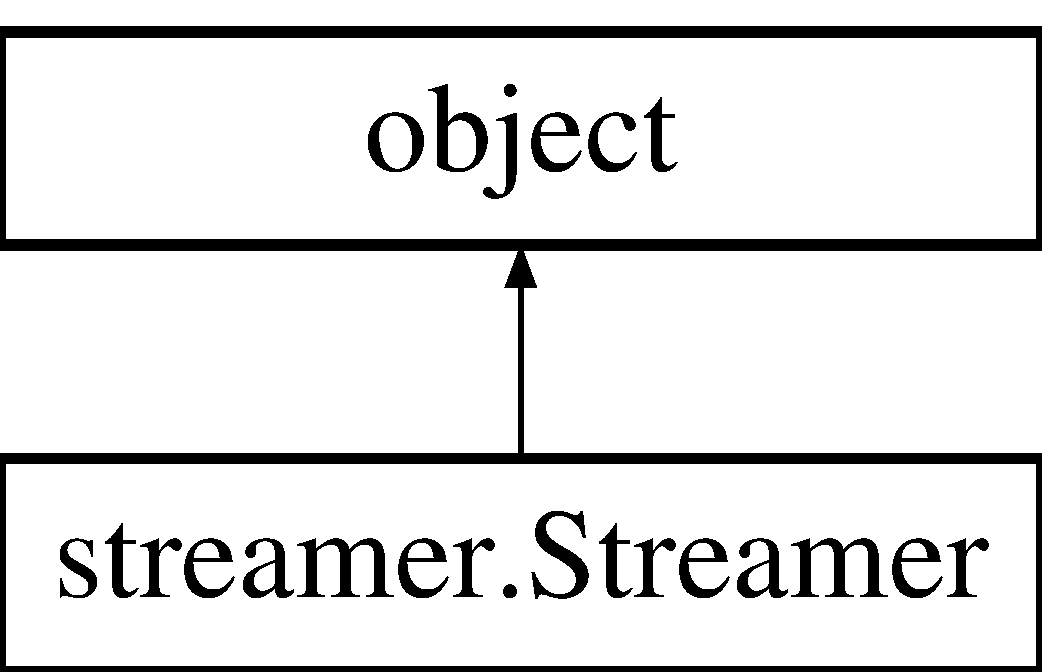
\includegraphics[height=2.000000cm]{classstreamer_1_1_streamer}
\end{center}
\end{figure}
\subsection*{Public Member Functions}
\begin{DoxyCompactItemize}
\item 
def \mbox{\hyperlink{classstreamer_1_1_streamer_aae063a4ecba841acd0f6994af01d59c2}{\+\_\+\+\_\+init\+\_\+\+\_\+}} (self)
\item 
def \mbox{\hyperlink{classstreamer_1_1_streamer_a23ddd6eaeab682bd4267c13b0d6ff45a}{exit\+\_\+handler}} (self)
\item 
def \mbox{\hyperlink{classstreamer_1_1_streamer_a2b946c06d88923c6e742c7cfeb50331b}{display\+\_\+status}} (self)
\item 
def \mbox{\hyperlink{classstreamer_1_1_streamer_adf219de2f5539f544a36ce625d3c265f}{process\+\_\+post}} (self, post, top\+Post=False)
\item 
def \mbox{\hyperlink{classstreamer_1_1_streamer_a17ac10d55adba12d6f2ba2bc842d0176}{stream\+\_\+step}} (self, hashtag, get\+Top\+Posts, step\+Index)
\item 
def \mbox{\hyperlink{classstreamer_1_1_streamer_a4fa871cd42320cd2df771d9844d1a67c}{start\+\_\+stream}} (self)
\end{DoxyCompactItemize}
\subsection*{Public Attributes}
\begin{DoxyCompactItemize}
\item 
\mbox{\hyperlink{classstreamer_1_1_streamer_a8277cc626d919a135a8c7f2b1c8d48b7}{config}}
\begin{DoxyCompactList}\small\item\em Login au compte Instagram du projet pour avoir accès à l\textquotesingle{}A\+PI. \end{DoxyCompactList}\item 
\mbox{\hyperlink{classstreamer_1_1_streamer_a9e80f10c0b27f7f88d401ce838975640}{Instagram\+A\+PI}}
\begin{DoxyCompactList}\small\item\em Connexion à l\textquotesingle{}A\+PI. \end{DoxyCompactList}\item 
\mbox{\Hypertarget{classstreamer_1_1_streamer_aa7493e40973e93c4d68e2859486132f7}\label{classstreamer_1_1_streamer_aa7493e40973e93c4d68e2859486132f7}} 
{\bfseries hashtags\+\_\+sponsor\+\_\+related}
\item 
\mbox{\Hypertarget{classstreamer_1_1_streamer_ae284273790497dd16b742451763b8c1e}\label{classstreamer_1_1_streamer_ae284273790497dd16b742451763b8c1e}} 
{\bfseries hashtags\+\_\+random}
\item 
\mbox{\hyperlink{classstreamer_1_1_streamer_ae7cbab4c93f54faa038805789506e167}{sql\+Client}}
\begin{DoxyCompactList}\small\item\em Calcul du temps d\textquotesingle{}exécution de la fonction. \end{DoxyCompactList}\item 
\mbox{\Hypertarget{classstreamer_1_1_streamer_a78e223c97e44e78fe8d165488e1a1891}\label{classstreamer_1_1_streamer_a78e223c97e44e78fe8d165488e1a1891}} 
{\bfseries n\+\_\+comments}
\end{DoxyCompactItemize}


\subsection{Detailed Description}
\begin{DoxyVerb}Streamer class.
\end{DoxyVerb}
 

\subsection{Constructor \& Destructor Documentation}
\mbox{\Hypertarget{classstreamer_1_1_streamer_aae063a4ecba841acd0f6994af01d59c2}\label{classstreamer_1_1_streamer_aae063a4ecba841acd0f6994af01d59c2}} 
\index{streamer\+::\+Streamer@{streamer\+::\+Streamer}!\+\_\+\+\_\+init\+\_\+\+\_\+@{\+\_\+\+\_\+init\+\_\+\+\_\+}}
\index{\+\_\+\+\_\+init\+\_\+\+\_\+@{\+\_\+\+\_\+init\+\_\+\+\_\+}!streamer\+::\+Streamer@{streamer\+::\+Streamer}}
\subsubsection{\texorpdfstring{\+\_\+\+\_\+init\+\_\+\+\_\+()}{\_\_init\_\_()}}
{\footnotesize\ttfamily def streamer.\+Streamer.\+\_\+\+\_\+init\+\_\+\+\_\+ (\begin{DoxyParamCaption}\item[{}]{self }\end{DoxyParamCaption})}

\begin{DoxyVerb}__init__ function.
\end{DoxyVerb}
 

\subsection{Member Function Documentation}
\mbox{\Hypertarget{classstreamer_1_1_streamer_a2b946c06d88923c6e742c7cfeb50331b}\label{classstreamer_1_1_streamer_a2b946c06d88923c6e742c7cfeb50331b}} 
\index{streamer\+::\+Streamer@{streamer\+::\+Streamer}!display\+\_\+status@{display\+\_\+status}}
\index{display\+\_\+status@{display\+\_\+status}!streamer\+::\+Streamer@{streamer\+::\+Streamer}}
\subsubsection{\texorpdfstring{display\+\_\+status()}{display\_status()}}
{\footnotesize\ttfamily def streamer.\+Streamer.\+display\+\_\+status (\begin{DoxyParamCaption}\item[{}]{self }\end{DoxyParamCaption})}

\begin{DoxyVerb}Affiche le statut du stream.

Args:
    (none)

Returns:
    (none)
\end{DoxyVerb}
 \mbox{\Hypertarget{classstreamer_1_1_streamer_a23ddd6eaeab682bd4267c13b0d6ff45a}\label{classstreamer_1_1_streamer_a23ddd6eaeab682bd4267c13b0d6ff45a}} 
\index{streamer\+::\+Streamer@{streamer\+::\+Streamer}!exit\+\_\+handler@{exit\+\_\+handler}}
\index{exit\+\_\+handler@{exit\+\_\+handler}!streamer\+::\+Streamer@{streamer\+::\+Streamer}}
\subsubsection{\texorpdfstring{exit\+\_\+handler()}{exit\_handler()}}
{\footnotesize\ttfamily def streamer.\+Streamer.\+exit\+\_\+handler (\begin{DoxyParamCaption}\item[{}]{self }\end{DoxyParamCaption})}

\begin{DoxyVerb}Ferme la session Postgre quand le script exit.

Args:
    (none)

Returns:
    (none)
\end{DoxyVerb}
 \mbox{\Hypertarget{classstreamer_1_1_streamer_adf219de2f5539f544a36ce625d3c265f}\label{classstreamer_1_1_streamer_adf219de2f5539f544a36ce625d3c265f}} 
\index{streamer\+::\+Streamer@{streamer\+::\+Streamer}!process\+\_\+post@{process\+\_\+post}}
\index{process\+\_\+post@{process\+\_\+post}!streamer\+::\+Streamer@{streamer\+::\+Streamer}}
\subsubsection{\texorpdfstring{process\+\_\+post()}{process\_post()}}
{\footnotesize\ttfamily def streamer.\+Streamer.\+process\+\_\+post (\begin{DoxyParamCaption}\item[{}]{self,  }\item[{}]{post,  }\item[{}]{top\+Post = {\ttfamily False} }\end{DoxyParamCaption})}

\begin{DoxyVerb}Traite le post Instagram et l'insère en base.

Args:
    post (dict) : le post Instagram à traiter.
    topPost (bool) : le post est-il récupéré en tant que TopPost sur Instagram ?

Returns:
    (none)
\end{DoxyVerb}
 \mbox{\Hypertarget{classstreamer_1_1_streamer_a4fa871cd42320cd2df771d9844d1a67c}\label{classstreamer_1_1_streamer_a4fa871cd42320cd2df771d9844d1a67c}} 
\index{streamer\+::\+Streamer@{streamer\+::\+Streamer}!start\+\_\+stream@{start\+\_\+stream}}
\index{start\+\_\+stream@{start\+\_\+stream}!streamer\+::\+Streamer@{streamer\+::\+Streamer}}
\subsubsection{\texorpdfstring{start\+\_\+stream()}{start\_stream()}}
{\footnotesize\ttfamily def streamer.\+Streamer.\+start\+\_\+stream (\begin{DoxyParamCaption}\item[{}]{self }\end{DoxyParamCaption})}

\begin{DoxyVerb}Démarre le stream.

Args:
    (none)

Returns:
    (none)
\end{DoxyVerb}
 \mbox{\Hypertarget{classstreamer_1_1_streamer_a17ac10d55adba12d6f2ba2bc842d0176}\label{classstreamer_1_1_streamer_a17ac10d55adba12d6f2ba2bc842d0176}} 
\index{streamer\+::\+Streamer@{streamer\+::\+Streamer}!stream\+\_\+step@{stream\+\_\+step}}
\index{stream\+\_\+step@{stream\+\_\+step}!streamer\+::\+Streamer@{streamer\+::\+Streamer}}
\subsubsection{\texorpdfstring{stream\+\_\+step()}{stream\_step()}}
{\footnotesize\ttfamily def streamer.\+Streamer.\+stream\+\_\+step (\begin{DoxyParamCaption}\item[{}]{self,  }\item[{}]{hashtag,  }\item[{}]{get\+Top\+Posts,  }\item[{}]{step\+Index }\end{DoxyParamCaption})}

\begin{DoxyVerb}Définit une étape du stream.

Args:
    hashtag (str) : le hashtag à streamer.
    getTopPosts (bool) : prendre en compte les Top Posts uniquement ou non.
    stepIndex (int) : le numéro de l'étape de stream.

Returns:
    (none)
\end{DoxyVerb}
 

\subsection{Member Data Documentation}
\mbox{\Hypertarget{classstreamer_1_1_streamer_a8277cc626d919a135a8c7f2b1c8d48b7}\label{classstreamer_1_1_streamer_a8277cc626d919a135a8c7f2b1c8d48b7}} 
\index{streamer\+::\+Streamer@{streamer\+::\+Streamer}!config@{config}}
\index{config@{config}!streamer\+::\+Streamer@{streamer\+::\+Streamer}}
\subsubsection{\texorpdfstring{config}{config}}
{\footnotesize\ttfamily streamer.\+Streamer.\+config}



Login au compte Instagram du projet pour avoir accès à l\textquotesingle{}A\+PI. 

\paragraph*{}\mbox{\Hypertarget{classstreamer_1_1_streamer_a9e80f10c0b27f7f88d401ce838975640}\label{classstreamer_1_1_streamer_a9e80f10c0b27f7f88d401ce838975640}} 
\index{streamer\+::\+Streamer@{streamer\+::\+Streamer}!Instagram\+A\+PI@{Instagram\+A\+PI}}
\index{Instagram\+A\+PI@{Instagram\+A\+PI}!streamer\+::\+Streamer@{streamer\+::\+Streamer}}
\subsubsection{\texorpdfstring{Instagram\+A\+PI}{InstagramAPI}}
{\footnotesize\ttfamily streamer.\+Streamer.\+Instagram\+A\+PI}



Connexion à l\textquotesingle{}A\+PI. 

\paragraph*{}\mbox{\Hypertarget{classstreamer_1_1_streamer_ae7cbab4c93f54faa038805789506e167}\label{classstreamer_1_1_streamer_ae7cbab4c93f54faa038805789506e167}} 
\index{streamer\+::\+Streamer@{streamer\+::\+Streamer}!sql\+Client@{sql\+Client}}
\index{sql\+Client@{sql\+Client}!streamer\+::\+Streamer@{streamer\+::\+Streamer}}
\subsubsection{\texorpdfstring{sql\+Client}{sqlClient}}
{\footnotesize\ttfamily streamer.\+Streamer.\+sql\+Client}



Calcul du temps d\textquotesingle{}exécution de la fonction. 

On veut que le temps minimal d\textquotesingle{}exécution soit de 10s. \#\#\# Questionnement de l\textquotesingle{}A\+PI sur les champs du post. \#\#\# Insertion dans la B\+DD. \#\#\# Si le client S\+QL ferme, on le réinstancie pour le rouvrir. \#\#\# 

The documentation for this class was generated from the following file\+:\begin{DoxyCompactItemize}
\item 
C\+:/\+Users/vberthelot/bulb/src/streamer.\+py\end{DoxyCompactItemize}

\hypertarget{classtrain_1_1_trainer}{}\section{train.\+Trainer Class Reference}
\label{classtrain_1_1_trainer}\index{train.\+Trainer@{train.\+Trainer}}
Inheritance diagram for train.\+Trainer\+:\begin{figure}[H]
\begin{center}
\leavevmode
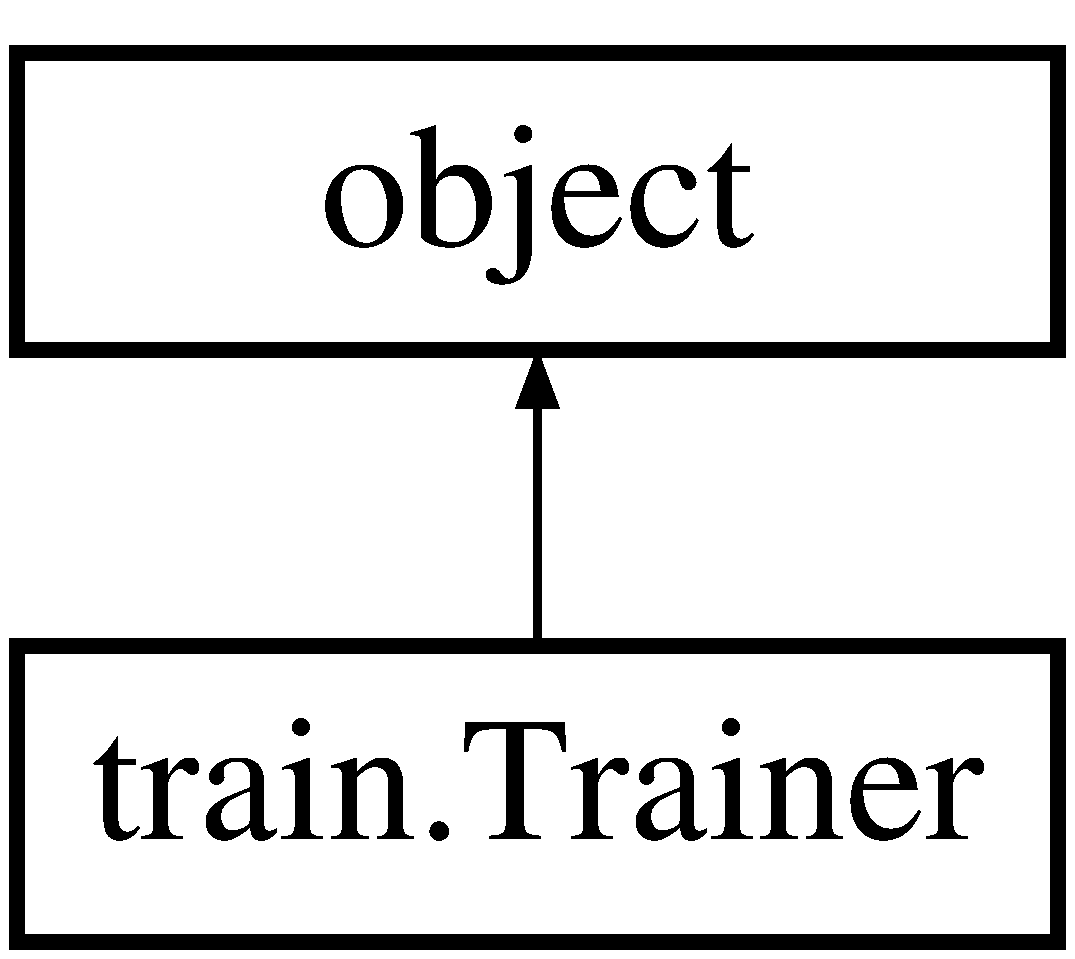
\includegraphics[height=2.000000cm]{classtrain_1_1_trainer}
\end{center}
\end{figure}
\subsection*{Public Member Functions}
\begin{DoxyCompactItemize}
\item 
def \mbox{\hyperlink{classtrain_1_1_trainer_a6b737f139c2c40d775b82f39ea836c90}{\+\_\+\+\_\+init\+\_\+\+\_\+}} (self, split\+\_\+ratio=0.\+75)
\item 
def \mbox{\hyperlink{classtrain_1_1_trainer_aa4cb6b5a4f8b87a958c9b6b62e6204b8}{build\+Users\+Model}} (self)
\item 
def \mbox{\hyperlink{classtrain_1_1_trainer_a9af45043f80d721cc77e5feaa80d589b}{train}} (self)
\item 
def \mbox{\hyperlink{classtrain_1_1_trainer_aff695c7da5cd408f7c89228edff8370d}{classify\+\_\+user}} (self)
\end{DoxyCompactItemize}
\subsection*{Public Attributes}
\begin{DoxyCompactItemize}
\item 
\mbox{\Hypertarget{classtrain_1_1_trainer_a04604b66388b32e9a6c0ba8c534c13e6}\label{classtrain_1_1_trainer_a04604b66388b32e9a6c0ba8c534c13e6}} 
{\bfseries key\+\_\+features}
\item 
\mbox{\Hypertarget{classtrain_1_1_trainer_a629ccd643b7db8dd8b6a06f67f39a0cc}\label{classtrain_1_1_trainer_a629ccd643b7db8dd8b6a06f67f39a0cc}} 
{\bfseries features\+\_\+array}
\item 
\mbox{\hyperlink{classtrain_1_1_trainer_ad50e395082044b5360a36a05228214e3}{labels}}
\begin{DoxyCompactList}\small\item\em On parcourt le tableau des utilisateurs pour leur assigner les features. \end{DoxyCompactList}\item 
\mbox{\Hypertarget{classtrain_1_1_trainer_ae77281ef8fd3170ab70fe27b3fb6ccb7}\label{classtrain_1_1_trainer_ae77281ef8fd3170ab70fe27b3fb6ccb7}} 
{\bfseries split\+\_\+ratio}
\item 
\mbox{\hyperlink{classtrain_1_1_trainer_adb7df426e58f065bdcdfd9289b5b779b}{user\+\_\+model}}
\begin{DoxyCompactList}\small\item\em On récupère toutes les features nécessaires pour entraîner le modèle. \end{DoxyCompactList}\item 
\mbox{\hyperlink{classtrain_1_1_trainer_ac54aaf4028ad0a283506e27d2b7f8118}{n\+\_\+split}}
\begin{DoxyCompactList}\small\item\em Si le modèle d\textquotesingle{}utilisateurs existe déjà, on l\textquotesingle{}ouvre. \end{DoxyCompactList}\end{DoxyCompactItemize}


\subsection{Detailed Description}
\begin{DoxyVerb}Classe d'entraînement du modèle de détection des influenceurs.
\end{DoxyVerb}
 

\subsection{Constructor \& Destructor Documentation}
\mbox{\Hypertarget{classtrain_1_1_trainer_a6b737f139c2c40d775b82f39ea836c90}\label{classtrain_1_1_trainer_a6b737f139c2c40d775b82f39ea836c90}} 
\index{train\+::\+Trainer@{train\+::\+Trainer}!\+\_\+\+\_\+init\+\_\+\+\_\+@{\+\_\+\+\_\+init\+\_\+\+\_\+}}
\index{\+\_\+\+\_\+init\+\_\+\+\_\+@{\+\_\+\+\_\+init\+\_\+\+\_\+}!train\+::\+Trainer@{train\+::\+Trainer}}
\subsubsection{\texorpdfstring{\+\_\+\+\_\+init\+\_\+\+\_\+()}{\_\_init\_\_()}}
{\footnotesize\ttfamily def train.\+Trainer.\+\_\+\+\_\+init\+\_\+\+\_\+ (\begin{DoxyParamCaption}\item[{}]{self,  }\item[{}]{split\+\_\+ratio = {\ttfamily 0.75} }\end{DoxyParamCaption})}

\begin{DoxyVerb}__init__ function. On définit aussi les features que l'on va utiliser pour l'étude.
\end{DoxyVerb}
 

\subsection{Member Function Documentation}
\mbox{\Hypertarget{classtrain_1_1_trainer_aa4cb6b5a4f8b87a958c9b6b62e6204b8}\label{classtrain_1_1_trainer_aa4cb6b5a4f8b87a958c9b6b62e6204b8}} 
\index{train\+::\+Trainer@{train\+::\+Trainer}!build\+Users\+Model@{build\+Users\+Model}}
\index{build\+Users\+Model@{build\+Users\+Model}!train\+::\+Trainer@{train\+::\+Trainer}}
\subsubsection{\texorpdfstring{build\+Users\+Model()}{buildUsersModel()}}
{\footnotesize\ttfamily def train.\+Trainer.\+build\+Users\+Model (\begin{DoxyParamCaption}\item[{}]{self }\end{DoxyParamCaption})}

\begin{DoxyVerb}Construit la liste des utilisateurs utile pour l'entrainement, avec les features correspondantes.

Args:
    (none)
Returns:
    (none)\end{DoxyVerb}
 \mbox{\Hypertarget{classtrain_1_1_trainer_aff695c7da5cd408f7c89228edff8370d}\label{classtrain_1_1_trainer_aff695c7da5cd408f7c89228edff8370d}} 
\index{train\+::\+Trainer@{train\+::\+Trainer}!classify\+\_\+user@{classify\+\_\+user}}
\index{classify\+\_\+user@{classify\+\_\+user}!train\+::\+Trainer@{train\+::\+Trainer}}
\subsubsection{\texorpdfstring{classify\+\_\+user()}{classify\_user()}}
{\footnotesize\ttfamily def train.\+Trainer.\+classify\+\_\+user (\begin{DoxyParamCaption}\item[{}]{self }\end{DoxyParamCaption})}

\begin{DoxyVerb}Classe un utilisateur Instagram selon le modèle déjà entraîné.

Args:
    (none)

Returns:
    (none)
\end{DoxyVerb}
 \mbox{\Hypertarget{classtrain_1_1_trainer_a9af45043f80d721cc77e5feaa80d589b}\label{classtrain_1_1_trainer_a9af45043f80d721cc77e5feaa80d589b}} 
\index{train\+::\+Trainer@{train\+::\+Trainer}!train@{train}}
\index{train@{train}!train\+::\+Trainer@{train\+::\+Trainer}}
\subsubsection{\texorpdfstring{train()}{train()}}
{\footnotesize\ttfamily def train.\+Trainer.\+train (\begin{DoxyParamCaption}\item[{}]{self }\end{DoxyParamCaption})}

\begin{DoxyVerb}Entraînement du modèle.

    Args:
(none)
    
    Returns:
(none)
\end{DoxyVerb}
 

\subsection{Member Data Documentation}
\mbox{\Hypertarget{classtrain_1_1_trainer_ad50e395082044b5360a36a05228214e3}\label{classtrain_1_1_trainer_ad50e395082044b5360a36a05228214e3}} 
\index{train\+::\+Trainer@{train\+::\+Trainer}!labels@{labels}}
\index{labels@{labels}!train\+::\+Trainer@{train\+::\+Trainer}}
\subsubsection{\texorpdfstring{labels}{labels}}
{\footnotesize\ttfamily train.\+Trainer.\+labels}



On parcourt le tableau des utilisateurs pour leur assigner les features. 

\paragraph*{}

Si l\textquotesingle{}utilisateur se trouve déjà dans le teableau, on n\textquotesingle{}a pas à réeffectuer le traitement. \#\#\# Récupère les features via la classe User. \#\#\# Sauvegarde du modèle d\textquotesingle{}utilisateurs. \#\#\# Assignation de la liste des features en tant que liste, et les labels correspondants. \#\#\# On mélange les résultats pour ne pas avoir toujours les mêmes répartitions coup sur coup. \#\#\# \mbox{\Hypertarget{classtrain_1_1_trainer_ac54aaf4028ad0a283506e27d2b7f8118}\label{classtrain_1_1_trainer_ac54aaf4028ad0a283506e27d2b7f8118}} 
\index{train\+::\+Trainer@{train\+::\+Trainer}!n\+\_\+split@{n\+\_\+split}}
\index{n\+\_\+split@{n\+\_\+split}!train\+::\+Trainer@{train\+::\+Trainer}}
\subsubsection{\texorpdfstring{n\+\_\+split}{n\_split}}
{\footnotesize\ttfamily train.\+Trainer.\+n\+\_\+split}



Si le modèle d\textquotesingle{}utilisateurs existe déjà, on l\textquotesingle{}ouvre. 

\paragraph*{}

Index du split. \#\#\# \mbox{\Hypertarget{classtrain_1_1_trainer_adb7df426e58f065bdcdfd9289b5b779b}\label{classtrain_1_1_trainer_adb7df426e58f065bdcdfd9289b5b779b}} 
\index{train\+::\+Trainer@{train\+::\+Trainer}!user\+\_\+model@{user\+\_\+model}}
\index{user\+\_\+model@{user\+\_\+model}!train\+::\+Trainer@{train\+::\+Trainer}}
\subsubsection{\texorpdfstring{user\+\_\+model}{user\_model}}
{\footnotesize\ttfamily train.\+Trainer.\+user\+\_\+model}



On récupère toutes les features nécessaires pour entraîner le modèle. 

\paragraph*{}

The documentation for this class was generated from the following file\+:\begin{DoxyCompactItemize}
\item 
src/train.\+py\end{DoxyCompactItemize}

\hypertarget{classuser_1_1_user}{}\section{user.\+User Class Reference}
\label{classuser_1_1_user}\index{user.\+User@{user.\+User}}
Inheritance diagram for user.\+User\+:\begin{figure}[H]
\begin{center}
\leavevmode
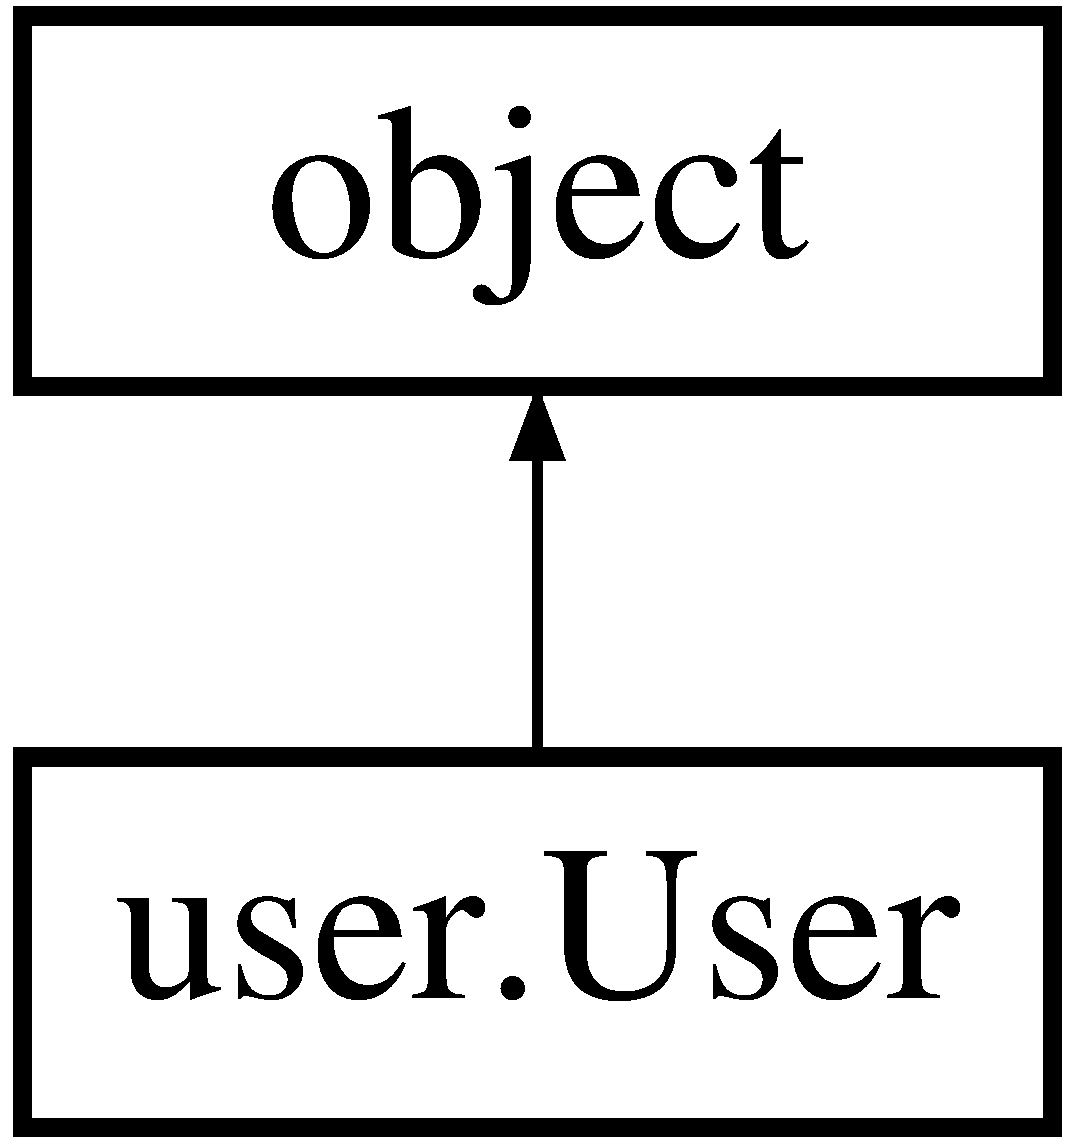
\includegraphics[height=2.000000cm]{classuser_1_1_user}
\end{center}
\end{figure}
\subsection*{Public Member Functions}
\begin{DoxyCompactItemize}
\item 
def \mbox{\hyperlink{classuser_1_1_user_a25681f18d7857cac8117612e68c92cc5}{\+\_\+\+\_\+init\+\_\+\+\_\+}} (self)
\item 
def \mbox{\hyperlink{classuser_1_1_user_a09bf41f6ea57ec2ce77fa616738d08bc}{get\+User\+Names}} (self, limit=0)
\item 
def \mbox{\hyperlink{classuser_1_1_user_a7dfe5ca7988fd34b0c801742a5aa84e6}{get\+User\+Info\+IG}} (self)
\item 
def \mbox{\hyperlink{classuser_1_1_user_a5b18648f492550fba80fd13478888d1d}{get\+User\+Info\+S\+QL}} (self)
\item 
def \mbox{\hyperlink{classuser_1_1_user_a8fb05076e464cc8df275207908fd30bc}{get\+Most\+Dominant\+Colour}} (self, image)
\item 
def \mbox{\hyperlink{classuser_1_1_user_a1876aea4aa2e915ff8e933910f2df6e4}{get\+Image\+Colorfulness}} (self, image)
\item 
def \mbox{\hyperlink{classuser_1_1_user_ab013b6d1535fe2b752a8eb5649018a1c}{get\+Contrast}} (self, img)
\item 
def \mbox{\hyperlink{classuser_1_1_user_a5269972e3c641c50202185b171fe904b}{get\+Brand\+Presence}} (self, post)
\item 
def \mbox{\hyperlink{classuser_1_1_user_a3fd64901698b59210a03be44ff5123e8}{get\+Brand\+Types}} (self, brands)
\item 
def \mbox{\hyperlink{classuser_1_1_user_ae21bbe88ed8f0421aba11b51df3fc03f}{get\+Comment\+Score}} (self, comment)
\item 
def \mbox{\hyperlink{classuser_1_1_user_a817542763611c0dd2d4ae4efc997f079}{create\+Comments\+Model}} (self)
\item 
def \mbox{\hyperlink{classuser_1_1_user_a91c0417fe409dae061a9acc84222e124}{process\+Word\+Comment}} (self, word)
\item 
def \mbox{\hyperlink{classuser_1_1_user_a2bf236a7cfb42cb97298c49d29330e69}{test\+Comment\+Score}} (self)
\end{DoxyCompactItemize}
\subsection*{Public Attributes}
\begin{DoxyCompactItemize}
\item 
\mbox{\hyperlink{classuser_1_1_user_a40419b31c47368b454fa2003b5df9307}{config}}
\begin{DoxyCompactList}\small\item\em L\textquotesingle{}utilisateur hérite de la classe {\ttfamily object}. \end{DoxyCompactList}\item 
\mbox{\Hypertarget{classuser_1_1_user_a22920e0da789e7da4462f98d18f0d5f1}\label{classuser_1_1_user_a22920e0da789e7da4462f98d18f0d5f1}} 
{\bfseries username}
\item 
\mbox{\hyperlink{classuser_1_1_user_adf4a399faa3ea66427ecf7cb8a1bbb89}{sql\+Client}}
\begin{DoxyCompactList}\small\item\em Instanciation du client S\+QL. \end{DoxyCompactList}\item 
\mbox{\hyperlink{classuser_1_1_user_ad3a0ba5c1d994eef3cc7a0c5de2bfa85}{n\+\_\+clusters}}
\begin{DoxyCompactList}\small\item\em Ici, on cherche à avoir la distorsion des k-\/means des couleurs du feed. \end{DoxyCompactList}\item 
\mbox{\hyperlink{classuser_1_1_user_a31bd1f48a5a64a4319d8d93beca49706}{lastpost}}
\begin{DoxyCompactList}\small\item\em Initialisation des features pour l\textquotesingle{}apprentissage. \end{DoxyCompactList}\item 
\mbox{\Hypertarget{classuser_1_1_user_a95227c69ec5585fd19625ffdb5c3b739}\label{classuser_1_1_user_a95227c69ec5585fd19625ffdb5c3b739}} 
{\bfseries frequency}
\item 
\mbox{\hyperlink{classuser_1_1_user_a7e0889f882283a613c48be7c1c5802cb}{engagement}}
\begin{DoxyCompactList}\small\item\em Initialisation des listes de stockage pour les métriques. \end{DoxyCompactList}\item 
\mbox{\Hypertarget{classuser_1_1_user_ab7e01826b02c1fd36fe40ec3ef122619}\label{classuser_1_1_user_ab7e01826b02c1fd36fe40ec3ef122619}} 
{\bfseries followings}
\item 
\mbox{\Hypertarget{classuser_1_1_user_a6c75e0121b5cd3810b18ba8bb5415731}\label{classuser_1_1_user_a6c75e0121b5cd3810b18ba8bb5415731}} 
{\bfseries followers}
\item 
\mbox{\Hypertarget{classuser_1_1_user_a1299fa6854061f717587f485cbd65e9d}\label{classuser_1_1_user_a1299fa6854061f717587f485cbd65e9d}} 
{\bfseries usermentions}
\item 
\mbox{\Hypertarget{classuser_1_1_user_abd0372db83f1098f7b0f2d135ce16e99}\label{classuser_1_1_user_abd0372db83f1098f7b0f2d135ce16e99}} 
{\bfseries brandpresence}
\item 
\mbox{\Hypertarget{classuser_1_1_user_abb534bea6556322d857746a2bbd8d1ba}\label{classuser_1_1_user_abb534bea6556322d857746a2bbd8d1ba}} 
{\bfseries brandtypes}
\item 
\mbox{\Hypertarget{classuser_1_1_user_a5dff9881f19c6e51a38ec00ad5023b52}\label{classuser_1_1_user_a5dff9881f19c6e51a38ec00ad5023b52}} 
{\bfseries commentscore}
\item 
\mbox{\hyperlink{classuser_1_1_user_a40a93b76c643c0eb076abc8ae0f15f31}{K}}
\begin{DoxyCompactList}\small\item\em Paramètres de fonctions maths, pour ajustement de scores. \end{DoxyCompactList}\item 
\mbox{\Hypertarget{classuser_1_1_user_a6d7d87038a73b8d70d9a42527c9327bb}\label{classuser_1_1_user_a6d7d87038a73b8d70d9a42527c9327bb}} 
{\bfseries K\+\_\+}
\item 
\mbox{\Hypertarget{classuser_1_1_user_ab533b4b4d7236b1c4a18a462605fa34d}\label{classuser_1_1_user_ab533b4b4d7236b1c4a18a462605fa34d}} 
{\bfseries B}
\item 
\mbox{\hyperlink{classuser_1_1_user_a6bd90421024505f3be18cab7f2b56dd8}{Instagram\+A\+PI}}
\begin{DoxyCompactList}\small\item\em Connexion à l\textquotesingle{}A\+PI. \end{DoxyCompactList}\item 
\mbox{\Hypertarget{classuser_1_1_user_a760c3a66bfca4082009586aa5b78f2da}\label{classuser_1_1_user_a760c3a66bfca4082009586aa5b78f2da}} 
{\bfseries colorfulness\+\_\+std}
\item 
\mbox{\Hypertarget{classuser_1_1_user_aea903db123f8c9cd65025aa76a4c0555}\label{classuser_1_1_user_aea903db123f8c9cd65025aa76a4c0555}} 
{\bfseries contrast\+\_\+std}
\item 
\mbox{\Hypertarget{classuser_1_1_user_aab2a5bfc38a04a549b34e9dd2e7216e5}\label{classuser_1_1_user_aab2a5bfc38a04a549b34e9dd2e7216e5}} 
{\bfseries colors}
\item 
\mbox{\Hypertarget{classuser_1_1_user_a52f95c80145dab806b28bf825223ca74}\label{classuser_1_1_user_a52f95c80145dab806b28bf825223ca74}} 
{\bfseries color\+\_\+distorsion}
\item 
\mbox{\Hypertarget{classuser_1_1_user_a9ddb37752ef26c665dba7d0fbbeb094e}\label{classuser_1_1_user_a9ddb37752ef26c665dba7d0fbbeb094e}} 
{\bfseries colors\+\_\+dispersion}
\item 
\mbox{\Hypertarget{classuser_1_1_user_ad680260b05eb361e7062950112676ae0}\label{classuser_1_1_user_ad680260b05eb361e7062950112676ae0}} 
{\bfseries label}
\end{DoxyCompactItemize}


\subsection{Detailed Description}
\begin{DoxyVerb}Classe utilisateur.
\end{DoxyVerb}
 

\subsection{Constructor \& Destructor Documentation}
\mbox{\Hypertarget{classuser_1_1_user_a25681f18d7857cac8117612e68c92cc5}\label{classuser_1_1_user_a25681f18d7857cac8117612e68c92cc5}} 
\index{user\+::\+User@{user\+::\+User}!\+\_\+\+\_\+init\+\_\+\+\_\+@{\+\_\+\+\_\+init\+\_\+\+\_\+}}
\index{\+\_\+\+\_\+init\+\_\+\+\_\+@{\+\_\+\+\_\+init\+\_\+\+\_\+}!user\+::\+User@{user\+::\+User}}
\subsubsection{\texorpdfstring{\+\_\+\+\_\+init\+\_\+\+\_\+()}{\_\_init\_\_()}}
{\footnotesize\ttfamily def user.\+User.\+\_\+\+\_\+init\+\_\+\+\_\+ (\begin{DoxyParamCaption}\item[{}]{self }\end{DoxyParamCaption})}

\begin{DoxyVerb}__init__ function.
\end{DoxyVerb}
 

\subsection{Member Function Documentation}
\mbox{\Hypertarget{classuser_1_1_user_a817542763611c0dd2d4ae4efc997f079}\label{classuser_1_1_user_a817542763611c0dd2d4ae4efc997f079}} 
\index{user\+::\+User@{user\+::\+User}!create\+Comments\+Model@{create\+Comments\+Model}}
\index{create\+Comments\+Model@{create\+Comments\+Model}!user\+::\+User@{user\+::\+User}}
\subsubsection{\texorpdfstring{create\+Comments\+Model()}{createCommentsModel()}}
{\footnotesize\ttfamily def user.\+User.\+create\+Comments\+Model (\begin{DoxyParamCaption}\item[{}]{self }\end{DoxyParamCaption})}

\begin{DoxyVerb}Crée le modèle de commentaires.

Args:
    (none)

Returns:
    (none)
\end{DoxyVerb}
 \mbox{\Hypertarget{classuser_1_1_user_a5269972e3c641c50202185b171fe904b}\label{classuser_1_1_user_a5269972e3c641c50202185b171fe904b}} 
\index{user\+::\+User@{user\+::\+User}!get\+Brand\+Presence@{get\+Brand\+Presence}}
\index{get\+Brand\+Presence@{get\+Brand\+Presence}!user\+::\+User@{user\+::\+User}}
\subsubsection{\texorpdfstring{get\+Brand\+Presence()}{getBrandPresence()}}
{\footnotesize\ttfamily def user.\+User.\+get\+Brand\+Presence (\begin{DoxyParamCaption}\item[{}]{self,  }\item[{}]{post }\end{DoxyParamCaption})}

\begin{DoxyVerb}Retourne les mentions utilisateur qui matchent avec les utilisateurs mentionnés dans la description du post.

Args:
    post (dict) : un post Instagram sous forme de dictionnaire.

Returns:
    (str[]) Le tableau contenant les marques détectées.
\end{DoxyVerb}
 \mbox{\Hypertarget{classuser_1_1_user_a3fd64901698b59210a03be44ff5123e8}\label{classuser_1_1_user_a3fd64901698b59210a03be44ff5123e8}} 
\index{user\+::\+User@{user\+::\+User}!get\+Brand\+Types@{get\+Brand\+Types}}
\index{get\+Brand\+Types@{get\+Brand\+Types}!user\+::\+User@{user\+::\+User}}
\subsubsection{\texorpdfstring{get\+Brand\+Types()}{getBrandTypes()}}
{\footnotesize\ttfamily def user.\+User.\+get\+Brand\+Types (\begin{DoxyParamCaption}\item[{}]{self,  }\item[{}]{brands }\end{DoxyParamCaption})}

\begin{DoxyVerb}Retourne les types de business que sont les 'marques' mentionnées à la fois dans la description du post et en mention utilisateur.

Args:
    brands (str[]) : le tableau des utilisateurs détectés.

Returns:
    (Counter) Le compteur de types de profils utilisateur (Blog, Photographe, Acteur, etc.), si le type de compte est 'Business' seulement.
\end{DoxyVerb}
 \mbox{\Hypertarget{classuser_1_1_user_ae21bbe88ed8f0421aba11b51df3fc03f}\label{classuser_1_1_user_ae21bbe88ed8f0421aba11b51df3fc03f}} 
\index{user\+::\+User@{user\+::\+User}!get\+Comment\+Score@{get\+Comment\+Score}}
\index{get\+Comment\+Score@{get\+Comment\+Score}!user\+::\+User@{user\+::\+User}}
\subsubsection{\texorpdfstring{get\+Comment\+Score()}{getCommentScore()}}
{\footnotesize\ttfamily def user.\+User.\+get\+Comment\+Score (\begin{DoxyParamCaption}\item[{}]{self,  }\item[{}]{comment }\end{DoxyParamCaption})}

\begin{DoxyVerb}Retourne le score de commentaire basé sur le modèle de commentaires.
Les commentaire les plus pertinents pour une photo (= dont les mots importants sont peu utilisés dans le modèle de commentaires) sont privilégiés.
Les commentaires les plus longs sont privilégiés.

Args:
    comment (str): le commentaire texte.

Returns:
    (int) Le score de qualité de commentaire, situé entre 0 et 1.
\end{DoxyVerb}
 \mbox{\Hypertarget{classuser_1_1_user_ab013b6d1535fe2b752a8eb5649018a1c}\label{classuser_1_1_user_ab013b6d1535fe2b752a8eb5649018a1c}} 
\index{user\+::\+User@{user\+::\+User}!get\+Contrast@{get\+Contrast}}
\index{get\+Contrast@{get\+Contrast}!user\+::\+User@{user\+::\+User}}
\subsubsection{\texorpdfstring{get\+Contrast()}{getContrast()}}
{\footnotesize\ttfamily def user.\+User.\+get\+Contrast (\begin{DoxyParamCaption}\item[{}]{self,  }\item[{}]{img }\end{DoxyParamCaption})}

\begin{DoxyVerb}Retourne le contraste global de l'image en passant par un calcul d'entropie.

Args:
    img (Image PIL) : l'image N&B qu'on considère pour l'étude (matrice d'entiers allant de 0 à 255).

Returns:
    (int) Le contraste de l'image.
\end{DoxyVerb}
 \mbox{\Hypertarget{classuser_1_1_user_a1876aea4aa2e915ff8e933910f2df6e4}\label{classuser_1_1_user_a1876aea4aa2e915ff8e933910f2df6e4}} 
\index{user\+::\+User@{user\+::\+User}!get\+Image\+Colorfulness@{get\+Image\+Colorfulness}}
\index{get\+Image\+Colorfulness@{get\+Image\+Colorfulness}!user\+::\+User@{user\+::\+User}}
\subsubsection{\texorpdfstring{get\+Image\+Colorfulness()}{getImageColorfulness()}}
{\footnotesize\ttfamily def user.\+User.\+get\+Image\+Colorfulness (\begin{DoxyParamCaption}\item[{}]{self,  }\item[{}]{image }\end{DoxyParamCaption})}

\begin{DoxyVerb}Retourne l'intensité colorimétrique de l'image.

Args:
        image (Image PIL) : l'image qu'on considère pour l'étude.

Returns:
        (int) L'intensité colorimétrique de l'image.
\end{DoxyVerb}
 \mbox{\Hypertarget{classuser_1_1_user_a8fb05076e464cc8df275207908fd30bc}\label{classuser_1_1_user_a8fb05076e464cc8df275207908fd30bc}} 
\index{user\+::\+User@{user\+::\+User}!get\+Most\+Dominant\+Colour@{get\+Most\+Dominant\+Colour}}
\index{get\+Most\+Dominant\+Colour@{get\+Most\+Dominant\+Colour}!user\+::\+User@{user\+::\+User}}
\subsubsection{\texorpdfstring{get\+Most\+Dominant\+Colour()}{getMostDominantColour()}}
{\footnotesize\ttfamily def user.\+User.\+get\+Most\+Dominant\+Colour (\begin{DoxyParamCaption}\item[{}]{self,  }\item[{}]{image }\end{DoxyParamCaption})}

\begin{DoxyVerb}Retourne la couleur dominante de l'image.

Args:
        image (Image PIL) : l'image qu'on considère pour l'étude.

Returns:
        (tuple) La couleur dominante de l'image dans le repère lab*.
\end{DoxyVerb}
 \mbox{\Hypertarget{classuser_1_1_user_a7dfe5ca7988fd34b0c801742a5aa84e6}\label{classuser_1_1_user_a7dfe5ca7988fd34b0c801742a5aa84e6}} 
\index{user\+::\+User@{user\+::\+User}!get\+User\+Info\+IG@{get\+User\+Info\+IG}}
\index{get\+User\+Info\+IG@{get\+User\+Info\+IG}!user\+::\+User@{user\+::\+User}}
\subsubsection{\texorpdfstring{get\+User\+Info\+I\+G()}{getUserInfoIG()}}
{\footnotesize\ttfamily def user.\+User.\+get\+User\+Info\+IG (\begin{DoxyParamCaption}\item[{}]{self }\end{DoxyParamCaption})}

\begin{DoxyVerb}Récupération des critères de l'utilisateur via l'API d'Instagram.
Utilisée lorsqu'on veut tester notre modèle en live, sur un utilisateur qui n'est pas forcément en base.

Args:
(none)

Returns:
(none)
\end{DoxyVerb}
 \mbox{\Hypertarget{classuser_1_1_user_a5b18648f492550fba80fd13478888d1d}\label{classuser_1_1_user_a5b18648f492550fba80fd13478888d1d}} 
\index{user\+::\+User@{user\+::\+User}!get\+User\+Info\+S\+QL@{get\+User\+Info\+S\+QL}}
\index{get\+User\+Info\+S\+QL@{get\+User\+Info\+S\+QL}!user\+::\+User@{user\+::\+User}}
\subsubsection{\texorpdfstring{get\+User\+Info\+S\+Q\+L()}{getUserInfoSQL()}}
{\footnotesize\ttfamily def user.\+User.\+get\+User\+Info\+S\+QL (\begin{DoxyParamCaption}\item[{}]{self }\end{DoxyParamCaption})}

\begin{DoxyVerb}On récupère les posts de l'utilisateur à partir de la BDD, et on en extrait les features nécessaires pour l'apprentissage.
L'intérêt de cette méthode est qu'on peut solliciter la BDD très vite par rapport à l'API Instagram, ce qui nous permet de faire un
apprentissage 'rapide'!
La méthode est cependant très similaire à `self.getUserInfoIG()`.

Args:
        (none)

Returns:
        (none)
\end{DoxyVerb}
 \mbox{\Hypertarget{classuser_1_1_user_a09bf41f6ea57ec2ce77fa616738d08bc}\label{classuser_1_1_user_a09bf41f6ea57ec2ce77fa616738d08bc}} 
\index{user\+::\+User@{user\+::\+User}!get\+User\+Names@{get\+User\+Names}}
\index{get\+User\+Names@{get\+User\+Names}!user\+::\+User@{user\+::\+User}}
\subsubsection{\texorpdfstring{get\+User\+Names()}{getUserNames()}}
{\footnotesize\ttfamily def user.\+User.\+get\+User\+Names (\begin{DoxyParamCaption}\item[{}]{self,  }\item[{}]{limit = {\ttfamily 0} }\end{DoxyParamCaption})}

\begin{DoxyVerb}Récupère les usernames des utilisateurs annotés.

Args:
limit (int) : La limite du nombre d'utilisateurs à retourner.

Returns:
(list) : la liste des noms d'utilisateur issus de la BDD.
\end{DoxyVerb}
 \mbox{\Hypertarget{classuser_1_1_user_a91c0417fe409dae061a9acc84222e124}\label{classuser_1_1_user_a91c0417fe409dae061a9acc84222e124}} 
\index{user\+::\+User@{user\+::\+User}!process\+Word\+Comment@{process\+Word\+Comment}}
\index{process\+Word\+Comment@{process\+Word\+Comment}!user\+::\+User@{user\+::\+User}}
\subsubsection{\texorpdfstring{process\+Word\+Comment()}{processWordComment()}}
{\footnotesize\ttfamily def user.\+User.\+process\+Word\+Comment (\begin{DoxyParamCaption}\item[{}]{self,  }\item[{}]{word }\end{DoxyParamCaption})}

\begin{DoxyVerb}Pré-processe le commentaire.

Args:
    word (str) : le mot.

Return:
    (str) Le mot pré-processé.
\end{DoxyVerb}
 \mbox{\Hypertarget{classuser_1_1_user_a2bf236a7cfb42cb97298c49d29330e69}\label{classuser_1_1_user_a2bf236a7cfb42cb97298c49d29330e69}} 
\index{user\+::\+User@{user\+::\+User}!test\+Comment\+Score@{test\+Comment\+Score}}
\index{test\+Comment\+Score@{test\+Comment\+Score}!user\+::\+User@{user\+::\+User}}
\subsubsection{\texorpdfstring{test\+Comment\+Score()}{testCommentScore()}}
{\footnotesize\ttfamily def user.\+User.\+test\+Comment\+Score (\begin{DoxyParamCaption}\item[{}]{self }\end{DoxyParamCaption})}

\begin{DoxyVerb}Tooling permettant de tester les scores des commentaires utilisateur.

Args:
    (none)

Returns:
    (none)
\end{DoxyVerb}
 

\subsection{Member Data Documentation}
\mbox{\Hypertarget{classuser_1_1_user_a40419b31c47368b454fa2003b5df9307}\label{classuser_1_1_user_a40419b31c47368b454fa2003b5df9307}} 
\index{user\+::\+User@{user\+::\+User}!config@{config}}
\index{config@{config}!user\+::\+User@{user\+::\+User}}
\subsubsection{\texorpdfstring{config}{config}}
{\footnotesize\ttfamily user.\+User.\+config}



L\textquotesingle{}utilisateur hérite de la classe {\ttfamily object}. 

\paragraph*{}

On charge les variables depuis le fichier de config. \#\#\# \mbox{\Hypertarget{classuser_1_1_user_a7e0889f882283a613c48be7c1c5802cb}\label{classuser_1_1_user_a7e0889f882283a613c48be7c1c5802cb}} 
\index{user\+::\+User@{user\+::\+User}!engagement@{engagement}}
\index{engagement@{engagement}!user\+::\+User@{user\+::\+User}}
\subsubsection{\texorpdfstring{engagement}{engagement}}
{\footnotesize\ttfamily user.\+User.\+engagement}



Initialisation des listes de stockage pour les métriques. 

\paragraph*{}

Timestamps et taux d\textquotesingle{}engagement\+: métriques immédiates. \#\#\# On récupère le code binaire des images en B\+DD, et on y opère les traitements \+: \#\#\#
\begin{DoxyItemize}
\item S\+TD du contraste \#\#\#
\item S\+TD de l\textquotesingle{}intensité colorimétrique \#\#\#
\item Distorsion des clusters de couleur \#\#\# On essaye d\textquotesingle{}avoir les images des posts afin de les traiter automatiquement et en extraire les features. \#\#\# Si erreur il y a, on passe à la suivante sans breaker le script. \#\#\# On récupère les octets de l\textquotesingle{}image. \#\#\# On convertit l\textquotesingle{}image en N\&B pour l\textquotesingle{}étude du contraste. \#\#\# On ajoute la couleur dominante du post pour une analyse colorimétrique. \#\#\# On récupère le taux de colorité de l\textquotesingle{}image, qu\textquotesingle{}on ajoute à la liste globale si cette première n\textquotesingle{}est pas nan. \#\#\# On récupère le taux de contraste de l\textquotesingle{}image, qu\textquotesingle{}on ajoute à la liste globale si cette première n\textquotesingle{}est pas nan. \#\#\# Pour l\textquotesingle{}instant on ne s\textquotesingle{}en sert pas, à ré-\/utiliser quand on s\textquotesingle{}intéressera à la détection des placements de produits. \#\#\# On parcourt les commentaires du post pour en extraire le \char`\"{}score de commentaires\char`\"{}. \#\#\# Si le nombre de commentaires est trop bas, on affecte des valeurs particulières. \#\#\# En effet, la variance d\textquotesingle{}une VA prend en arguments deux points de données minimum. \#\#\# Dernière phase\+: on affecte les variables d\textquotesingle{}instance (= features) une fois que tous les critères ont été traités. \#\#\# 
\end{DoxyItemize}\mbox{\Hypertarget{classuser_1_1_user_a6bd90421024505f3be18cab7f2b56dd8}\label{classuser_1_1_user_a6bd90421024505f3be18cab7f2b56dd8}} 
\index{user\+::\+User@{user\+::\+User}!Instagram\+A\+PI@{Instagram\+A\+PI}}
\index{Instagram\+A\+PI@{Instagram\+A\+PI}!user\+::\+User@{user\+::\+User}}
\subsubsection{\texorpdfstring{Instagram\+A\+PI}{InstagramAPI}}
{\footnotesize\ttfamily user.\+User.\+Instagram\+A\+PI}



Connexion à l\textquotesingle{}A\+PI. 

\paragraph*{}\mbox{\Hypertarget{classuser_1_1_user_a40a93b76c643c0eb076abc8ae0f15f31}\label{classuser_1_1_user_a40a93b76c643c0eb076abc8ae0f15f31}} 
\index{user\+::\+User@{user\+::\+User}!K@{K}}
\index{K@{K}!user\+::\+User@{user\+::\+User}}
\subsubsection{\texorpdfstring{K}{K}}
{\footnotesize\ttfamily user.\+User.\+K}



Paramètres de fonctions maths, pour ajustement de scores. 

\paragraph*{}\mbox{\Hypertarget{classuser_1_1_user_a31bd1f48a5a64a4319d8d93beca49706}\label{classuser_1_1_user_a31bd1f48a5a64a4319d8d93beca49706}} 
\index{user\+::\+User@{user\+::\+User}!lastpost@{lastpost}}
\index{lastpost@{lastpost}!user\+::\+User@{user\+::\+User}}
\subsubsection{\texorpdfstring{lastpost}{lastpost}}
{\footnotesize\ttfamily user.\+User.\+lastpost}



Initialisation des features pour l\textquotesingle{}apprentissage. 

On essaye d\textquotesingle{}extraire les features du profil Instagram.

\paragraph*{}

\paragraph*{}

Si il y a une erreur, on pass (on ne veut pas break e script en cas de re-\/promptage). \#\#\# Les {\ttfamily time.\+sleep} préviennent des erreurs 503, dues à une sollicitation trop soudaine de l\textquotesingle{}A\+PI Instagram. \#\#\# On initialise le temps de départ pour mesurer le temps d\textquotesingle{}exécution global. \#\#\# On questionne l\textquotesingle{}A\+PI à propos du nom d\textquotesingle{}utilisateur, cela nous retourne l\textquotesingle{}utilisateur en entier. \#\#\# On récupère le feed entier de l\textquotesingle{}utilisateur, afin d\textquotesingle{}analyser certaines métriques. \#\#\# On initialise les listes utiles pour l\textquotesingle{}étude. \#\#\# On affiche la longueur du feed retourné par l\textquotesingle{}A\+PI. \#\#\# On boucle sur le feed afin d\textquotesingle{}en extraire les données pertinentes pour le calcul de nos features. \#\#\# On prend 50 posts du feed pour ne pas avoir un temps d\textquotesingle{}éxécution trop long. \#\#\# T\+O\+DO\+: demander à l\textquotesingle{}A\+PI de ne pas récupérer l\textquotesingle{}intégralité des posts de l\textquotesingle{}utilisateur, mais simplement les 50 premiers. \#\#\# On affiche l\textquotesingle{}état de progression de l\textquotesingle{}analyse. \#\#\# Si le serveur renvoie une erreur (notamment 503), on attend 1 minute avant de renvoyer une requête. \#\#\# On ajoute le timestamp du post pour les analyses de fréquence. \#\#\# Si l\textquotesingle{}utilisateur n\textquotesingle{}a pas de followers, on considère que le taux d\textquotesingle{}engagement est 0 (au lieu d\textquotesingle{}infini). \#\#\# Pourcentage du taux d\textquotesingle{}engagement. \#\#\# On distingue plusieurs cas\+: celui où il y a commentaires et likes, celui où il en manque un des deux, et celui où il n\textquotesingle{}y a rien. \#\#\# On ajoute le taux d\textquotesingle{}engagement du post à la liste de taux d\textquotesingle{}engagement. \#\#\# On récupère le code binaire des images en B\+DD, et on y opère les traitements \+: \#\#\#
\begin{DoxyItemize}
\item S\+TD du contraste \#\#\#
\item S\+TD de l\textquotesingle{}intensité colorimétrique \#\#\#
\item Distorsion des clusters de couleur \#\#\# Depuis le J\+S\+ON de réponse de l\textquotesingle{}A\+PI, on récupère l\textquotesingle{}adresse U\+RL de la plus petite image. \#\#\# On fait une requête H\+T\+T\+P.\+G\+ET sur l\textquotesingle{}adresse récupérée, puis on entrait les octets de l\textquotesingle{}image en réponse. \#\#\# On convertit l\textquotesingle{}image en N\&B pour l\textquotesingle{}étude du contraste. \#\#\# On ajoute la couleur dominante du post pour une analyse colorimétrique. \#\#\# On récupère le taux de colorité de l\textquotesingle{}image, qu\textquotesingle{}on ajoute à la liste globale si cette première n\textquotesingle{}est pas nan. \#\#\# On récupère le taux de contraste de l\textquotesingle{}image, qu\textquotesingle{}on ajoute à la liste globale si cette première n\textquotesingle{}est pas nan. \#\#\# Fetch les marques détectées dans les posts. \#\#\# On récupère le score de commentaires sur tout le feed de l\textquotesingle{}utilisateur. \#\#\# On cherche tous les commentaires retournés dans la variable {\ttfamily comments\+\_\+server}. \#\#\# On ne prend que les 10 premier commentaires pour chaque post. \#\#\# Si la personne qui commente est l\textquotesingle{}auteur du post, alors on ignore le commentaire. \#\#\# Si on a une erreur, on attend une minute avant de recommencer l\textquotesingle{}opération. \#\#\# Assignation des critères et affichage des résultats. \#\#\# 
\end{DoxyItemize}\mbox{\Hypertarget{classuser_1_1_user_ad3a0ba5c1d994eef3cc7a0c5de2bfa85}\label{classuser_1_1_user_ad3a0ba5c1d994eef3cc7a0c5de2bfa85}} 
\index{user\+::\+User@{user\+::\+User}!n\+\_\+clusters@{n\+\_\+clusters}}
\index{n\+\_\+clusters@{n\+\_\+clusters}!user\+::\+User@{user\+::\+User}}
\subsubsection{\texorpdfstring{n\+\_\+clusters}{n\_clusters}}
{\footnotesize\ttfamily user.\+User.\+n\+\_\+clusters}



Ici, on cherche à avoir la distorsion des k-\/means des couleurs du feed. 

\paragraph*{}

Parfois, on peut avoir que une ou deux couleurs outputées du k-\/mean. \#\#\# Si on a une erreur, on baisse le nombre de clusters jusqu\textquotesingle{}à ce que le k-\/mean puisse être opéré. \#\#\# \mbox{\Hypertarget{classuser_1_1_user_adf4a399faa3ea66427ecf7cb8a1bbb89}\label{classuser_1_1_user_adf4a399faa3ea66427ecf7cb8a1bbb89}} 
\index{user\+::\+User@{user\+::\+User}!sql\+Client@{sql\+Client}}
\index{sql\+Client@{sql\+Client}!user\+::\+User@{user\+::\+User}}
\subsubsection{\texorpdfstring{sql\+Client}{sqlClient}}
{\footnotesize\ttfamily user.\+User.\+sql\+Client}



Instanciation du client S\+QL. 

\paragraph*{}

The documentation for this class was generated from the following file\+:\begin{DoxyCompactItemize}
\item 
src/user.\+py\end{DoxyCompactItemize}

%--- End generated contents ---

% Index
\backmatter
\newpage
\phantomsection
\clearemptydoublepage
\addcontentsline{toc}{chapter}{Index}
\printindex

\end{document}
